\documentclass[12pt,a4paper]{article}

% Packages
\usepackage[utf8]{vietnam}
\usepackage[vietnamese]{babel}
\usepackage{graphicx}
\usepackage{amsmath}
\usepackage{amssymb}
\usepackage{booktabs}
\usepackage{longtable}
\usepackage{hyperref}
\usepackage{geometry}
\usepackage{fancyhdr}
\usepackage{listings}
\usepackage{xcolor}
\usepackage{caption}
\usepackage{subcaption}
\usepackage{float}
\usepackage{enumitem}

% Page setup
\geometry{left=2.5cm, right=2.5cm, top=3cm, bottom=3cm}
\pagestyle{fancy}
\fancyhf{}
\fancyhead[L]{\leftmark}
\fancyhead[R]{\thepage}
\renewcommand{\headrulewidth}{0.4pt}

% Hyperref setup
\hypersetup{
    colorlinks=true,
    linkcolor=blue,
    filecolor=magenta,      
    urlcolor=cyan,
    citecolor=green,
}

% Listings setup for code
\lstset{
    basicstyle=\ttfamily\small,
    breaklines=true,
    frame=single,
    backgroundcolor=\color{gray!10},
    numbers=left,
    numberstyle=\tiny\color{gray},
    keywordstyle=\color{blue},
    commentstyle=\color{green!60!black},
    stringstyle=\color{red},
}

% Title information
\title{\textbf{BÁO CÁO KỸ THUẬT}\\
\Large Phân tích Thời tiết và Chất lượng Không khí\\
Thành phố Hồ Chí Minh năm 2023}

\author{
    \textbf{Tên nhóm:} [AIT2006-2-3.3]\\
    \textbf{Thành viên:}\\
    \begin{tabular}{ll}
        1. & [Nguyễn Gia Phát - 24022424]\\
        2. & [Nguyễn Bá An    - 24022246]\\
        3. & [Lê Mạnh Cường   - 24022276]\\
    \end{tabular}
}

\date{\textbf{Ngày nộp:} 19 tháng 12 năm 2025\\
\textbf{Commit Hash:} \texttt{bf1067f}}

\begin{document}

\maketitle
\thispagestyle{empty}

\newpage
\tableofcontents
\newpage

% ============================================================
\section{Thông tin cơ bản}
% ============================================================

\subsection{Thông tin dự án}
\begin{itemize}[leftmargin=*]
    \item \textbf{Tên dự án:} Weather \& Air Quality Analysis – Ho Chi Minh City 2023
    \item \textbf{Tên nhóm:} [AIT2006-2-3.3]
    \item \textbf{Năm dữ liệu:} 2023
    \item \textbf{Phạm vi:} Thành phố Hồ Chí Minh, Việt Nam
    \item \textbf{Ngày nộp:} 19 tháng 12 năm 2025
    \item \textbf{Commit hash:} \texttt{bf1067f} - branch Main
\end{itemize}

\subsection{Thành viên nhóm}
\begin{table}[H]
\centering
\begin{tabular}{clc}
\toprule
\textbf{STT} & \textbf{Họ và tên} & \textbf{MSSV} \\
\midrule
1 & [Nguyễn Gia Phát] & [24022424] \\
2 & [Nguyễn Bá An] & [24022246] \\
3 & [Lê Mạnh Cường] & [24022276] \\
\bottomrule
\end{tabular}
\caption{Danh sách thành viên nhóm}
\end{table}

% ============================================================
\section{Giới thiệu và Tổng quan Dữ liệu}
% ============================================================

\subsection{Bối cảnh và Mục tiêu}
Dự án này thực hiện phân tích toàn diện về dữ liệu thời tiết và chất lượng không khí tại Thành phố Hồ Chí Minh trong năm 2023. Mục tiêu chính bao gồm:

\begin{itemize}
    \item Làm sạch, chuẩn hóa và kiểm tra chất lượng dữ liệu thô
    \item Tạo các chỉ số tổng hợp theo ngày, tuần và tháng
    \item Trực quan hóa các xu hướng và mối quan hệ giữa các biến
    \item Dự báo nồng độ PM2.5 sử dụng mô hình học máy
    \item Phát hiện các giá trị bất thường trong nồng độ PM2.5
\end{itemize}

\subsection{Nguồn dữ liệu}

\subsubsection{Dữ liệu Thời tiết}
\begin{itemize}
    \item \textbf{Nguồn:} Meteostat (thông qua API)
    \item \textbf{Tần suất:} Dữ liệu theo giờ được tổng hợp thành dữ liệu ngày
    \item \textbf{Biến chính:}
    \begin{itemize}
        \item Nhiệt độ: trung bình (tavg), tối thiểu (tmin), tối đa (tmax)
        \item Lượng mưa (prcp) tính bằng mm
        \item Tốc độ gió (wspd) tính bằng km/h
        \item Áp suất khí quyển (pres) tính bằng hPa
        \item Chỉ số UV (uv\_index\_max, uv\_index\_clear\_sky\_max)
    \end{itemize}
\end{itemize}

\subsubsection{Dữ liệu Chất lượng Không khí}
\begin{itemize}
    \item \textbf{Nguồn:} Open-Meteo Air Quality API
    \item \textbf{Tần suất:} Dữ liệu theo giờ (8760 quan sát)
    \item \textbf{Biến chính:}
    \begin{itemize}
        \item PM2.5: Bụi mịn có đường kính $\leq$ 2.5 $\mu$m
        \item PM10: Bụi mịn có đường kính $\leq$ 10 $\mu$m
        \item $NO_2$ (nitrogen\_dioxide): Khí nitrogen dioxide
        \item $SO_2$ (sulphur\_dioxide): Khí sulfur dioxide
        \item $O_3$ (ozone): Khí ozone
        \item CO (carbon\_monoxide): Khí carbon monoxide
    \end{itemize}
\end{itemize}

\subsection{Đặc điểm chính của Dữ liệu}

\subsubsection{Phạm vi thời gian}
\begin{itemize}
    \item \textbf{Khoảng thời gian:} 01/01/2023 -- 31/12/2023 (365 ngày)
    \item \textbf{Độ phủ dữ liệu:} 100\% (365/365 ngày hợp lệ sau QA)
    \item \textbf{Dữ liệu theo giờ:} 8760 quan sát (365 ngày × 24 giờ)
\end{itemize}

\subsubsection{Thống kê mô tả ban đầu}
\begin{table}[H]
\centering
\small
\begin{tabular}{lcccc}
\toprule
\textbf{Biến} & \textbf{Trung bình} & \textbf{Độ lệch chuẩn} & \textbf{Min} & \textbf{Max} \\
\midrule
\multicolumn{5}{l}{\textbf{Thời tiết}} \\
Nhiệt độ TB (°C) & 28.68 & 1.26 & 25.10 & 32.50 \\
Nhiệt độ min (°C) & 25.33 & 1.52 & 21.00 & 29.00 \\
Nhiệt độ max (°C) & 33.33 & 1.68 & 27.00 & 38.00 \\
Lượng mưa (mm/ngày) & 6.04 & 7.96 & 0.00 & 56.10 \\
Tốc độ gió (km/h) & 10.33 & 3.61 & 3.90 & 21.50 \\
Áp suất (hPa) & 1009.64 & 1.93 & 1004.40 & 1015.30 \\
\midrule
\multicolumn{5}{l}{\textbf{Chất lượng không khí}} \\
PM2.5 ($\mu$g/m³) & 24.13 & 8.55 & 8.97 & 54.45 \\
PM10 ($\mu$g/m³) & 35.80 & 12.53 & 13.07 & 79.53 \\

\bottomrule
\end{tabular}
\caption{Thống kê mô tả dữ liệu đã làm sạch (365 ngày năm 2023)}
\end{table}

\textit{\small chi tiết các biến còn lại xem trong resample.ipynb}
% ============================================================
\section{Làm sạch và Chuẩn hóa Dữ liệu}
\label{sec:qa}
% ============================================================

\subsection{Quy tắc Kiểm tra Chất lượng (QA Rules)}

\subsubsection{QA cho Dữ liệu Thời tiết}
Pipeline làm sạch dữ liệu thời tiết được thực hiện trong notebook \texttt{clean\_data.ipynb} với các quy tắc sau:

\begin{enumerate}
    \item \textbf{Kiểm tra giá trị thiếu:}
    \begin{itemize}
        \item Đánh dấu các quan sát có giá trị null/NaN
    \end{itemize}
    
    \item \textbf{Kiểm tra phạm vi vật lý:}
    \begin{itemize}
        \item Nhiệt độ: $-80°C \leq T \leq 60°C$
        \item Lượng mưa: $\geq 0$ mm
        \item Tốc độ gió: $\geq 0$ km/h
        \item Áp suất: $870 \leq P \leq 1100$ hPa
    \end{itemize}
    
    \item \textbf{Kiểm tra tính nhất quán:}
    \begin{itemize}
        \item $T_{min} \leq T_{avg} \leq T_{max}$
    \end{itemize}
    
    \item \textbf{Xử lý giá trị bất thường:}
    \begin{itemize}
        \item Đánh dấu (flag) thay vì loại bỏ hoàn toàn
    \end{itemize}
\end{enumerate}

\subsubsection{QA cho Dữ liệu Chất lượng Không khí}
\begin{enumerate}
    \item \textbf{Kiểm tra giá trị thiếu:}
    \begin{itemize}
        \item Đánh dấu các giờ/ngày có dữ liệu thiếu
        \item Tính tỷ lệ độ phủ dữ liệu
    \end{itemize}
    
    \item \textbf{Kiểm tra phạm vi:}
    \begin{itemize}
        \item Giá trị âm
        \item PM2.5: $0 \leq PM_{2.5} \leq 500$ $\mu$g/m³
        \item PM10: $0 \leq PM_{10} \leq 1000$ $\mu$g/m³
        \item PM2.5 $\leq$ PM10 (tính nhất quán vật lý)
        \item Chỉ số UV: $0 \leq UV \leq 15$
    \end{itemize}
    
    \item \textbf{Kiểm tra sự thay đổi đột ngột:}
    \begin{itemize}
        \item Phát hiện các thay đổi đột ngột giữa các quan sát liên tiếp
    \end{itemize}
\end{enumerate}

\subsection{Tác động của QA}

\subsubsection{Kết quả QA Dữ liệu Thời tiết}
\begin{table}[H]
\centering
\begin{tabular}{lcccc}
\toprule
\textbf{Loại lỗi} & \textbf{Số lượng} & \textbf{Tỷ lệ (\%)} & \textbf{Xử lý} \\
\midrule
Giá trị thiếu (nhiệt độ) & 0 & 0.0 & Đánh dấu flag \\
Giá trị thiếu (mưa/gió/áp suất) & 0 & 0.0 & Đánh dấu flag \\
Nhiệt độ ngoài phạm vi vật lý & 0 & 0.0 & Đánh dấu flag \\
Mưa âm hoặc gió âm & 0 & 0.0 & Đánh dấu flag \\
Áp suất ngoài 870-1100 hPa & 0 & 0.0 & Đánh dấu flag \\
Tmin > Tmax (không nhất quán) & 0 & 0.0 & Đánh dấu flag \\
Khoảng cách thời gian > 1 ngày & 0 & 0.0 & Đánh dấu flag \\
\midrule
\textbf{Tổng quan sát hợp lệ} & 365 & 100.0 &  \\
\bottomrule
\end{tabular}
\caption{Kết quả QA cho dữ liệu thời tiết ngày - Chất lượng dữ liệu xuất sắc}
\end{table}

\subsubsection{Kết quả QA Dữ liệu Chất lượng Không khí}
\begin{table}[H]
\centering
\begin{tabular}{lcccc}
\toprule
\textbf{Loại lỗi} & \textbf{Số lượng} & \textbf{Tỷ lệ (\%)} & \textbf{Xử lý} \\
\midrule
Giá trị thiếu (pollutants) & 0 & 0.00 & Đánh dấu flag \\
Giá trị âm không hợp lý & 0 & 0.00 & Thay bằng 0 \\
PM2.5 > PM10 & 4 & 0.05 & Auto-cap PM2.5 \\
UV index âm & 0 & 0.00 & Thay bằng 0 \\
UV index ngoài [0, 15] & 0 & 0.00 & Đánh dấu flag \\
PM2.5 ngoài [0, 500] µg/m³ & 0 & 0.00 & Đánh dấu flag \\
PM10 ngoài [0, 1000] µg/m³ & 0 & 0.00 & Đánh dấu flag \\
Duplicate timestamp & 0 & 0.00 & Giữ bản ghi đầu \\
Khoảng cách > 1 giờ & 0 & 0.00 & Đánh dấu flag \\
\midrule
\textbf{Tổng quan sát} & 8760 & 100.0 & \\
\bottomrule
\end{tabular}
\caption{Kết quả QA cho dữ liệu chất lượng không khí theo giờ (8760 quan sát)}
\end{table}

\subsection{Chuẩn hóa}

\subsection{Đồng bộ thời gian và đơn vị}

\subsubsection{Chuẩn hóa múi giờ}
\begin{itemize}
    \item Tất cả dữ liệu thời tiết và chất lượng không khí được chuẩn hóa về múi giờ UTC+7 (Việt Nam)
    \item Định dạng thời gian: \texttt{YYYY-MM-DD HH:MM:SS} cho dữ liệu theo giờ, \texttt{YYYY-MM-DD} cho dữ liệu ngày
\end{itemize}

\subsubsection{Resample về daily trước khi nối}
\begin{itemize}
    \item Dữ liệu chất lượng không khí (theo giờ) được tổng hợp thành dữ liệu ngày bằng các phép tính phù hợp:
    \begin{itemize}
        \item PM2.5, PM10: trung bình ngày (mean)
        \item UV index: giá trị tối đa trong ngày (max)
        \item Các chất khí (NO2, SO2, O3, CO): trung bình ngày (mean)
    \end{itemize}
    \item Dữ liệu thời tiết đã ở độ phân giải ngày từ nguồn
    \item Sau đó nối (merge) hai bộ dữ liệu theo cột \texttt{date}
\end{itemize}

\subsubsection{Thống nhất đơn vị cho các biến}
\begin{itemize}
    \item \textbf{Nhiệt độ:} °C (Celsius)
    \item \textbf{Lượng mưa:} mm (millimet)
    \item \textbf{Tốc độ gió:} km/h (kilomet/giờ)
    \item \textbf{Áp suất:} hPa (hectopascal)
    \item \textbf{Nồng độ bụi:} $\mu$g/m³ (microgram/mét khối)
    \item \textbf{Chỉ số UV:} không đơn vị (index, 0-15)
    \item \textbf{Tên cột:} Thống nhất theo snake\_case (\texttt{temp\_mean}, \texttt{pm2\_5}, \texttt{wspd}, etc.)
\end{itemize}

% ============================================================
\section{Tổng hợp và Thống kê}
% ============================================================

\subsection{Bảng Tổng hợp Chỉ số Chính}

Các chỉ số được tổng hợp từ dữ liệu thô theo các mức độ khác nhau (ngày, tuần, tháng) để hỗ trợ phân tích xu hướng và mối quan hệ.

\subsubsection{Tổng hợp Chỉ số Thời tiết}

\begin{table}[H]
\centering
\small
\begin{tabular}{lcccc}
\toprule
\textbf{Chỉ số} & \textbf{Trung bình} & \textbf{Min} & \textbf{Max} & \textbf{Mô tả} \\
\midrule
Nhiệt độ TB (°C) & 28.68 & 25.10 & 32.50 & Nhiệt độ trung bình ngày \\
Lượng mưa (mm) & 6.04 & 0.00 & 56.10 & Tổng lượng mưa ngày \\
Tốc độ gió (km/h) & 10.33 & 3.90 & 21.50 & Gió trung bình ngày \\
Áp suất (hPa) & 1009.64 & 1004.40 & 1015.30 & Áp suất khí quyển TB \\
\bottomrule
\end{tabular}
\caption{Tổng hợp các chỉ số thời tiết chính năm 2023}
\end{table}

\subsubsection{Tổng hợp Chỉ số Chất lượng Không khí}

\begin{table}[H]
\centering
\small
\begin{tabular}{lcccc}
\toprule
\textbf{Chỉ số} & \textbf{Trung bình} & \textbf{P50} & \textbf{P95} & \textbf{Ngưỡng WHO} \\
\midrule
PM2.5 ($\mu$g/m³) & 24.13 & 23.19 & 39.00 & 15 (24h) \\
PM10 ($\mu$g/m³) & 35.80 & 34.27 & 58.12 & 45 (24h) \\
NO$_2$ ($\mu$g/m³) & 28.93 & -- & -- & 25 (24h) \\
SO$_2$ ($\mu$g/m³) & 20.69 & -- & -- & 40 (24h) \\
O$_3$ ($\mu$g/m³) & 52.91 & -- & -- & 100 (8h) \\
CO ($\mu$g/m³) & 455.20 & -- & -- & 4000 (24h) \\
\bottomrule
\end{tabular}
\caption{Tổng hợp các chỉ số chất lượng không khí chính năm 2023}
\end{table}

\subsection{Tổng hợp theo Ngày}

Dữ liệu theo giờ từ hai nguồn (thời tiết và chất lượng không khí) được tổng hợp thành dữ liệu ngày thông qua các phép toán thống kê phù hợp với đặc trưng của từng biến:

\begin{itemize}
    \item \textbf{Nhiệt độ:} Được tính toán bằng giá trị trung bình, trung vị (p50), phân vị thứ 95 (p95), cùng với giá trị tối thiểu và tối đa trong ngày. Các chỉ số này giúp nắm bắt xu hướng trung tâm và biên độ dao động nhiệt.
    
    \item \textbf{Lượng mưa:} Sử dụng tổng lượng mưa tích lũy trong ngày (mm) và đếm số giờ có mưa đáng kể ($\geq$1mm). Đây là các chỉ số quan trọng để đánh giá cường độ và tần suất mưa.
    
    \item \textbf{Tốc độ gió:} Tính giá trị trung bình ngày, phản ánh điều kiện khuếch tán khí quyển. Gió mạnh giúp giảm nồng độ ô nhiễm thông qua cơ chế vận chuyển và khuếch tán.
    
    \item \textbf{Áp suất khí quyển:} Bao gồm giá trị trung bình và độ lệch chuẩn. Áp suất cao thường liên quan đến thời tiết ổn định và điều kiện bất lợi cho khuếch tán ô nhiễm.
    
    \item \textbf{Chất lượng không khí (PM2.5, PM10):} Sử dụng ba chỉ số chính:
    \begin{itemize}
        \item Giá trị trung bình ngày: Phản ánh mức độ ô nhiễm trung bình
        \item Phân vị thứ 95 (p95): Thể hiện mức độ ô nhiễm đỉnh trong ngày
        \item Số ngày vượt ngưỡng WHO: Đếm số ngày PM2.5 > 25 $\mu$g/m³ và PM10 > 50 $\mu$g/m³
    \end{itemize}
    
    \item \textbf{Chỉ số UV:} Giá trị trung bình và tối đa trong ngày, quan trọng cho cảnh báo sức khỏe và nguy cơ bỏng rạy.
\end{itemize}

\textbf{Phương pháp tổng hợp:} Các chỉ số được tính toán tự động bằng thuật toán resample theo chu kỳ ngày (daily), tuần (weekly), và tháng (monthly), đảm bảo tính nhất quán và khả năng tái sản xuất.

\subsection{Tổng hợp theo Tuần và Tháng}

Pipeline trong notebook \texttt{resample.ipynb} tạo các bảng tổng hợp:

\subsubsection{Chỉ số Tuần (\texttt{data\_weekly.csv})}
Các chỉ số được tính cho mỗi tuần (Monday--Sunday):
\begin{itemize}
    \item Nhiệt độ trung bình, p50, p95, min, max
    \item Tổng lượng mưa, số ngày mưa $\geq$ 1mm
    \item Tốc độ gió trung bình, áp suất trung bình và độ lệch chuẩn
    \item PM2.5 và PM10: p95, số ngày vượt ngưỡng
    \item Chỉ số UV trung bình và tối đa
\end{itemize}

\subsubsection{Chỉ số Tháng (\texttt{data\_monthly.csv})}
Tính toán tương tự cho từng tháng trong năm 2023.

\textbf{Bảng số liệu theo tháng cho các chỉ số chính:}

\begin{table}[H]
\centering
\small
\begin{tabular}{lrrrrr}
\toprule
\textbf{Tháng} & \textbf{Nhiệt độ TB} & \textbf{PM2.5 TB} & \textbf{PM2.5 P95} & \textbf{Mưa tổng} & \textbf{Gió TB} \\
 & \textbf{(°C)} & \textbf{($\mu$g/m³)} & \textbf{($\mu$g/m³)} & \textbf{(mm)} & \textbf{(km/h)} \\
\midrule
Tháng 1  & 27.25 & 30.91 & 51.49 & 83.5  & 9.17  \\
Tháng 2  & 28.30 & 21.72 & 33.17 & 9.3   & 9.52  \\
Tháng 3  & 28.44 & 19.12 & 25.70 & 3.1   & 10.73 \\
Tháng 4  & 30.50 & 24.10 & 41.71 & 58.7  & 11.22 \\
Tháng 5  & 29.98 & 24.59 & 35.62 & 233.7 & 10.94 \\
Tháng 6  & 29.14 & 28.39 & 42.60 & 353.1 & 11.61 \\
Tháng 7  & 28.12 & 19.95 & 30.49 & 422.6 & 12.17 \\
Tháng 8  & 29.20 & 19.61 & 26.29 & 237.1 & 15.03 \\
Tháng 9  & 27.98 & 21.52 & 34.04 & 334.4 & 11.14 \\
Tháng 10 & 28.04 & 26.17 & 36.87 & 347.3 & 6.65  \\
Tháng 11 & 28.42 & 29.28 & 48.03 & 97.6  & 7.50  \\
Tháng 12 & 28.80 & 24.21 & 35.67 & 25.6  & 8.18  \\
\midrule
\textbf{Trung bình} & \textbf{28.68} & \textbf{24.13} & \textbf{36.81} & \textbf{183.8} & \textbf{10.32} \\
\bottomrule
\end{tabular}
\caption{Số liệu thống kê theo tháng cho các chỉ số chính năm 2023}
\label{tab:monthly_data}
\end{table}

\textbf{Nhận xét:}
\begin{itemize}
    \item \textbf{PM2.5:} Cao nhất vào tháng 1 (30.91 $\mu$g/m³), thấp nhất tháng 3 và 8 ($\sim$19 $\mu$g/m³)
    \item \textbf{Mưa:} Mùa mưa chính từ tháng 5-10 với đỉnh tháng 7 (422.6mm)
    \item \textbf{Gió:} Mạnh nhất tháng 8 (15.03 km/h), yếu nhất tháng 10 (6.65 km/h)
    \item \textbf{Mối tương quan:} Tháng có mưa nhiều + gió mạnh thì PM2.5 thấp (tháng 7, 8, 9)
\end{itemize}

\subsubsection{Chỉ số Tháng có Chỉ mục (\texttt{data\_monthly\_indexed.csv})}
Chuẩn hóa các giá trị tháng với tháng đầu tiên (January) = 100:
\[
\text{Index}_i = \frac{\text{Value}_i}{\text{Value}_{\text{Jan}}} \times 100
\]

\subsection{Định nghĩa Chỉ số}

Bảng \ref{tab:indicators} liệt kê đầy đủ các chỉ số tổng hợp được sử dụng trong phân tích, bao gồm ý nghĩa, phương pháp tính toán và ngưỡng tham khảo từ các tiêu chuẩn quốc tế.

\begin{table}[H]
\centering
\small
\begin{tabular}{p{4cm}p{5.5cm}p{1.8cm}p{2.2cm}}
\toprule
\textbf{Chỉ số} & \textbf{Mô tả} & \textbf{Đơn vị} & \textbf{Ngưỡng} \\
\midrule
\multicolumn{4}{l}{\textit{\textbf{Chỉ số Thời tiết}}} \\
\midrule
Nhiệt độ trung bình & Giá trị trung bình nhiệt độ trong kỳ & °C & - \\
Nhiệt độ trung vị (P50) & Giá trị trung vị (50\% quan sát) & °C & - \\
Nhiệt độ P95 & Phân vị thứ 95 (nhiệt cao) & °C & >32°C \\
Nhiệt độ tối thiểu & Nhiệt độ thấp nhất ghi nhận & °C & <10°C \\
Nhiệt độ tối đa & Nhiệt độ cao nhất ghi nhận & °C & >40°C \\
\midrule
Tổng lượng mưa & Tổng lượng mưa tích lũy & mm & >100mm/tháng \\
Số ngày mưa & Ngày có mưa $\geq$1mm & ngày & >10/tháng \\
\midrule
Tốc độ gió TB & Tốc độ gió trung bình & km/h & >50 \\
\midrule
Áp suất TB & Áp suất khí quyển trung bình & hPa & <1000 \\
Áp suất độ lệch chuẩn & Biến động áp suất (chỉ số bất ổn) & hPa & >5 \\
\midrule
\multicolumn{4}{l}{\textit{\textbf{Chỉ số Chất lượng Không khí}}} \\
\midrule
PM2.5 trung bình & Nồng độ bụi mịn PM2.5 TB & $\mu$g/m³ & >15 (WHO) \\
PM2.5 P95 & Phân vị thứ 95 của PM2.5 & $\mu$g/m³ & >25 (WHO) \\
Ngày PM2.5 vượt WHO & Số ngày PM2.5 > 25 $\mu$g/m³ & ngày & >7/tháng \\
\midrule
PM10 trung bình & Nồng độ bụi thô PM10 TB & $\mu$g/m³ & >45 (WHO) \\
PM10 P95 & Phân vị thứ 95 của PM10 & $\mu$g/m³ & >50 (WHO) \\
Ngày PM10 vượt WHO & Số ngày PM10 > 50 $\mu$g/m³ & ngày & >7/tháng \\
\midrule
Chỉ số UV trung bình & Mức độ bức xạ UV TB & chỉ số & >6 (cao) \\
Chỉ số UV tối đa & Mức độ UV cao nhất & chỉ số & >11 (nguy hiểm) \\
\bottomrule
\end{tabular}
\caption{Định nghĩa và ngưỡng tham khảo cho các chỉ số tổng hợp}
\label{tab:indicators}
\end{table}
\textit{\small Lưu ý: Một số ngưỡng (tốc độ gió, áp suất, và nồng độ trung bình PM) được sử dụng với mục đích tham khảo và so sánh tương đối, do các khuyến nghị quốc tế thường áp dụng cho trung bình dài hạn (năm).}

\textbf{Giải thích các thuật ngữ:}
\begin{itemize}
    \item \textbf{Trung bình (Mean):} Tổng các giá trị chia cho số quan sát, phản ánh xu hướng trung tâm của dữ liệu
    \item \textbf{Trung vị (P50/Median):} Giá trị ở giữa khi sắp xếp dữ liệu, bền vững hơn trung bình với giá trị ngoại lai
    \item \textbf{Phân vị 95 (P95):} Giá trị mà 95\% quan sát thấp hơn, dùng để xác định giá trị cực đoan
    \item \textbf{Ngưỡng tham khảo:} Dựa trên WHO Air Quality Guidelines 2021, WMO standards, và QCVN Việt Nam
\end{itemize}

\textbf{Lưu ý:} 
\begin{itemize}
    \item Các chỉ số được tính toán tự động từ dữ liệu thô thông qua pipeline xử lý chuẩn hóa
    \item Kết quả được lưu trong các file: \texttt{data\_weekly.csv}, \texttt{data\_monthly.csv}, \texttt{data\_monthly\_indexed.csv}
    \item Bảng chi tiết về phương pháp tính toán có trong file \texttt{indicators\_documentation.csv}
\end{itemize}

% ============================================================
\section{Trực quan hóa}
% ============================================================

\subsection{Xu hướng Thời gian}

\subsubsection{Hình 1: Diễn biến PM2.5 theo thời gian (ngày)}

\textbf{Câu hỏi:} Nồng độ PM2.5 biến đổi như thế nào theo thời gian và mối liên hệ với nhiệt độ và lượng mưa?

\begin{figure}[H]
\centering
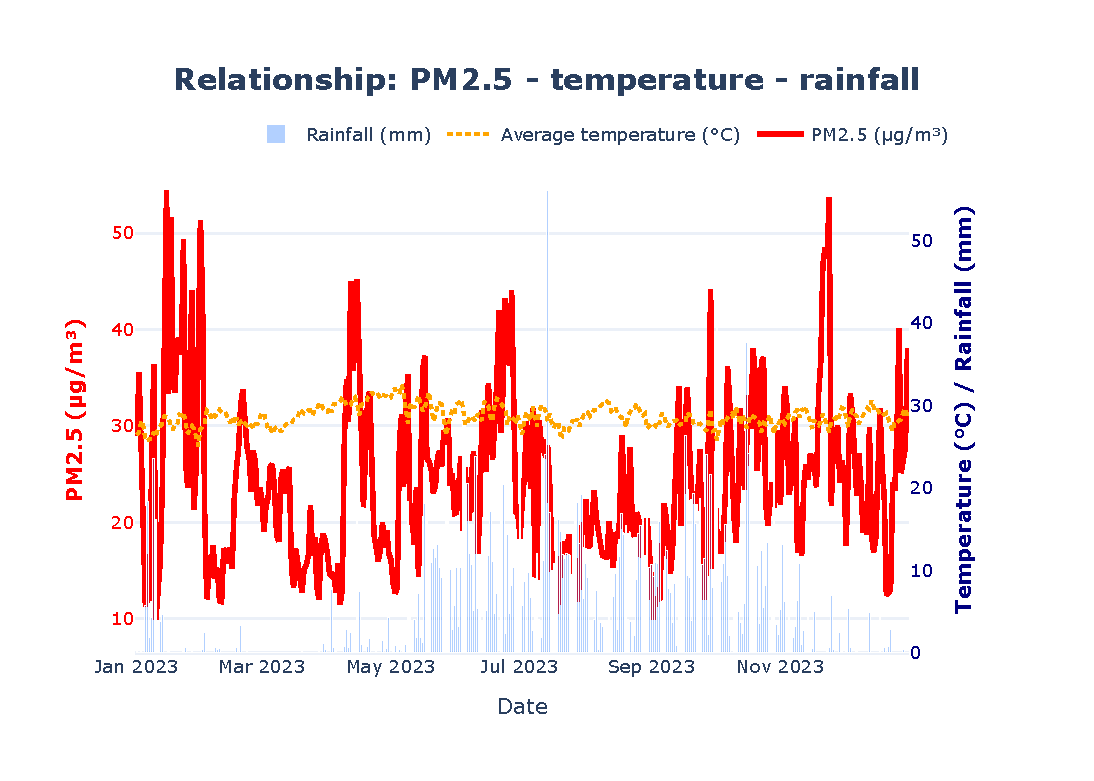
\includegraphics[width=\textwidth]{../figures/pm25-temp-rain.pdf}
\caption{Diễn biến PM2.5 (đường đỏ, $\mu$g/m³), Nhiệt độ trung bình (đường cam, °C), và Lượng mưa (thanh xanh, mm) theo ngày năm 2023}
\label{fig:pm_temp_rain_daily}
\end{figure}

\textbf{Phân tích chi tiết theo mùa (Đặc trưng khí hậu Nam Bộ: Mùa Khô và Mùa Mưa)}

Để hiểu rõ biểu đồ này, chúng ta cần chia thời gian thành 2 giai đoạn điển hình của khí hậu Nam Bộ: Mùa Khô và Mùa Mưa.

\textbf{Giai đoạn 1: Mùa Khô (Tháng 1 - Tháng 4 và quay lại vào Tháng 11)}

\begin{itemize}
    \item \textbf{Dữ liệu quan sát:}
    \begin{itemize}
        \item \textbf{Lượng mưa:} Các cột màu xanh gần như biến mất hoặc rất thấp, cho thấy tình trạng khô hạn kéo dài
        \item \textbf{PM2.5:} Đường màu đỏ dao động cực mạnh với biên độ lớn. Nhiều đỉnh nhọn (spikes) vượt rõ ngưỡng 50 $\mu$g/m³, thường xuyên ở mức 30-35 $\mu$g/m³
        \item \textbf{Nhiệt độ:} Tăng dần từ tháng 1 và đạt đỉnh nóng gắt vào tháng 4-5
    \end{itemize}
    
    \item \textbf{Phát hiện:} Đây là giai đoạn chất lượng không khí tệ nhất trong năm
\end{itemize}

\textbf{Giai đoạn 2: Mùa Mưa (Tháng 5 - Tháng 10)}

\begin{itemize}
    \item \textbf{Dữ liệu quan sát:}
    \begin{itemize}
        \item \textbf{Lượng mưa:} Mật độ các cột xanh dày đặc, xuất hiện liên tục với cường độ cao
        \item \textbf{PM2.5:} Đường màu đỏ có xu hướng hạ thấp nền chung. Mặc dù vẫn có dao động, nhưng các đỉnh nhọn ít vượt quá 30 $\mu$g/m³ và phần lớn duy trì ở mức trung bình 20 $\mu$g/m³
        \item \textbf{Nhiệt độ:} Giảm nhẹ do tác động làm mát của mưa
    \end{itemize}
    
    \item \textbf{Phát hiện:} Mùa mưa tương ứng với giai đoạn chất lượng không khí được cải thiện rõ rệt
\end{itemize}

\textbf{Giải thích Logic \& Cơ chế Khoa học}

Tại sao lại có sự phân hóa này ở TP.HCM? Dưới đây là lời giải thích cho các mối liên hệ tìm thấy:

\textbf{A. Mối tương quan nghịch giữa Mưa và Bụi (Cơ chế Rửa trôi)}

Biểu đồ cho thấy quy luật: \textbf{Mưa càng nhiều, Bụi càng giảm.}

\begin{itemize}
    \item \textbf{Cơ chế "Wet Deposition" (Lắng đọng ướt):} Tại TP.HCM, những cơn mưa rào lớn vào buổi chiều đóng vai trò như một hệ thống lọc khí không lồ. Các hạt mưa rơi xuống sẽ va chạm và cuốn theo hạt bụi PM2.5 lơ lửng, kéo chúng xuống mặt đất và cống thoát nước
    
    \item \textbf{Ngăn chặn bụi tái sinh:} Mưa làm ướt mặt đường và đất, ngăn cản bụi tồn đọng ở tầng thấp bị đưa lên không khí (một nguồn ô nhiễm lớn tại các đô thị đang xây dựng như TP.HCM)
\end{itemize}

\textbf{B. Tại sao Mùa Khô ô nhiễm lại tăng vọt? (Cơ chế Khí tượng Tĩnh)}

Vào các tháng 1, 2 và 11, 12, dù trời nắng đẹp nhưng chỉ số bụi (đường đỏ) lại cao nhất. Nguyên nhân nằm ở sự ổn định của khí quyển:

\begin{itemize}
    \item \textbf{Nghịch nhiệt (Thermal Inversion):} Vào ban đêm và sáng sớm mùa khô, lớp không khí sát đất lạnh hơn lớp không khí bên trên. Điều này tạo ra một "cái nắp" vô hình, nhốt toàn bộ khí bụi từ xe cộ và hoạt động công nghiệp ở tầng thấp, không cho chúng khuếch tán lên cao
    
    \item \textbf{Thiếu gió:} Gió yếu trong giai đoạn này khiến bụi không thể thổi bay đi xa, mà cứ tích tụ dần ngày qua ngày trong lòng thành phố
\end{itemize}

\textbf{C. Vai trò của Nhiệt độ}

\begin{itemize}
    \item Đường nhiệt độ (màu vàng) tại TP.HCM khá ổn định và dao động trong khoảng hẹp quanh năm (25-35°C). Điều này loại trừ nguyên nhân liên quan đến đốt nhiên liệu sưởi ấm (khác với Hà Nội hay các nước ôn đới)
    
    \item Do đó, sự biến thiên của PM2.5 trên biểu đồ này hoàn toàn bị chi phối bởi chế độ mưa và gió, chứ không phải do thay đổi nguồn thải theo nhiệt độ
\end{itemize}

\textbf{Kết luận}

Biểu đồ cung cấp bằng chứng thực nghiệm rõ ràng cho TP.HCM:

\begin{enumerate}
    \item \textbf{Thiên nhiên là máy lọc khí tốt nhất:} Sự xuất hiện của mưa (các cột xanh) là yếu tố chính giúp kiểm hãm nồng độ PM2.5
    
    \item \textbf{Cảnh báo sức khỏe:} Người dân cần đặc biệt đề phòng vào Mùa Khô (Tháng 11 đến Tháng 4 năm sau). Dù trời không mưa, nhìn về quan sát trời "đẹp" nhưng thực tế không hề có quan sát thiên nhiên hỗ trợ cơ chế làm sạch. Đó là lúc không khí "đầm đặc" bụi mịn nhất
\end{enumerate}

\subsubsection{Hình 2: Dashboard phân tích PM2.5 theo mức mưa và gió}

\textbf{Câu hỏi:} PM2.5 thay đổi như thế nào theo các mức độ mưa và tốc độ gió khác nhau?

\begin{figure}[H]
\centering
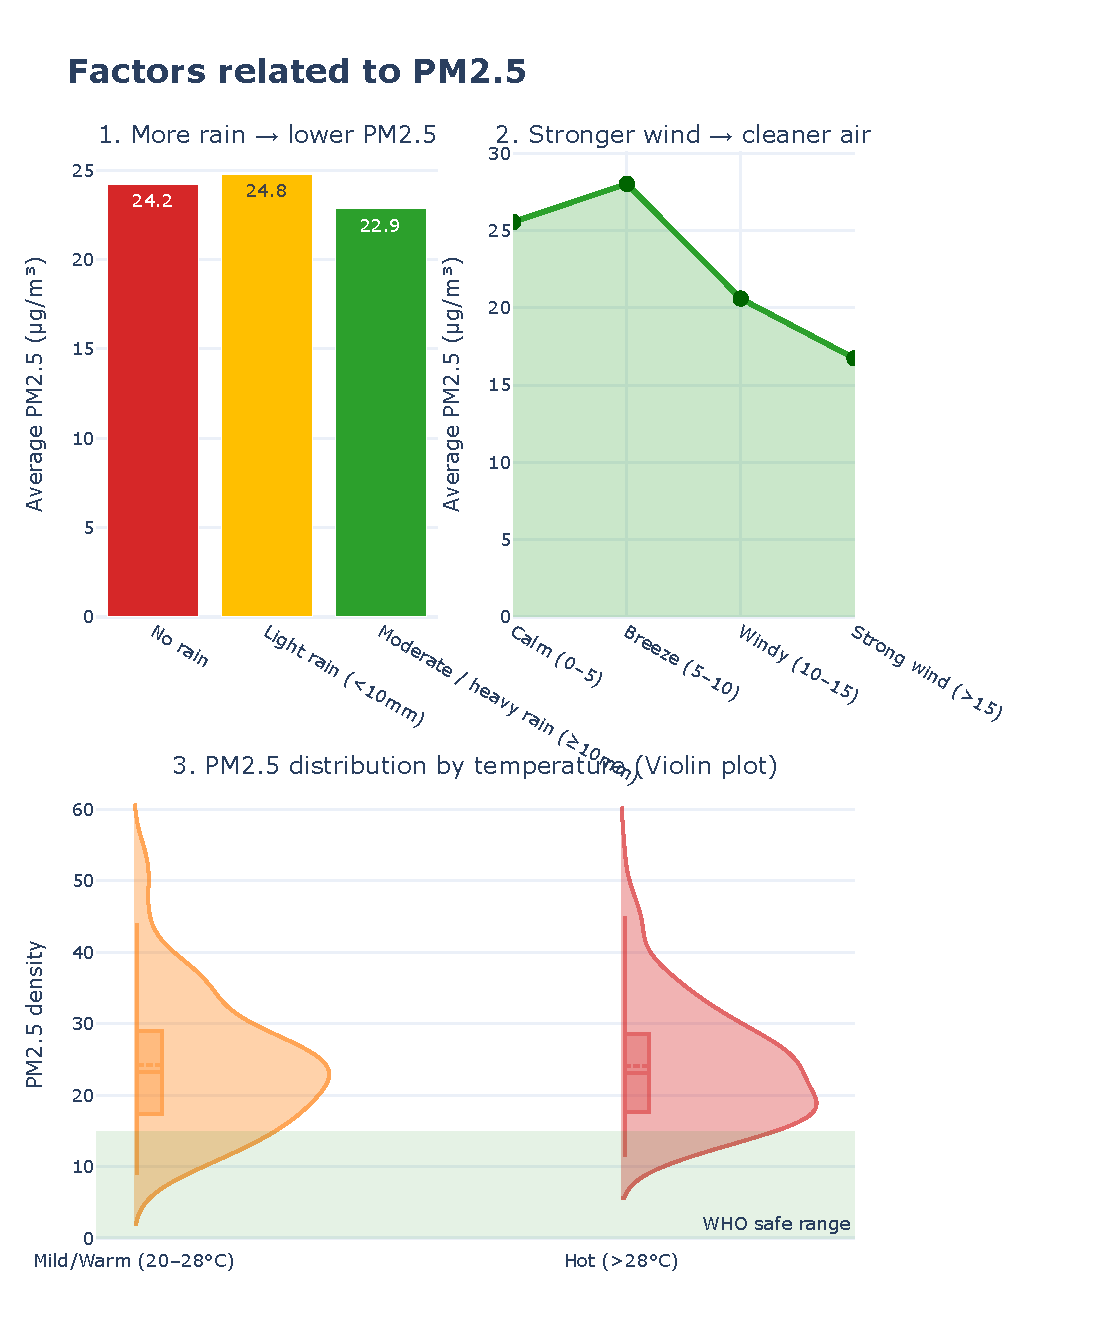
\includegraphics[width=\textwidth]{../figures/dashboard_rain_wind_temp.pdf}
\caption{Phân tích PM2.5 theo phân loại mưa, gió và nhiệt độ}
\label{fig:temp_rain}
\end{figure}

\textbf{Phân tích định lượng theo yếu tố:}

\begin{enumerate}
    \item \textbf{Vai trò của Gió - Phát hiện phi tuyến:}
    \begin{itemize}
        \item Gió yếu (<5 km/h): PM2.5 trung bình 25.2 $\mu$g/m³
        \item Gió vừa (5-10 km/h): PM2.5 tăng lên 28.1 $\mu$g/m³ (cao nhất)
        \item Gió mạnh (>10-15 km/h): PM2.5 giảm mạnh xuống 19.5 $\mu$g/m³
    \end{itemize}
    
    \textit{Giải thích:} Gió yếu chỉ đủ để nâng bụi từ bề mặt lên không khí nhưng không đủ mạnh để khuếch tán ra ngoài khu vực, gây tích tụ cục bộ. Chỉ khi tốc độ gió vượt ngưỡng $\sim$10 km/h, cơ chế khuếch tán theo chiều ngang và thẳng đứng mới hoạt động hiệu quả.
    
    \item \textbf{Hiệu ứng ngưỡng của Mưa:}
    \begin{itemize}
        \item Không mưa: PM2.5 = 24.3 $\mu$g/m³
        \item Mưa nhỏ (<10mm): PM2.5 = 24.8 $\mu$g/m³ (tăng nhẹ 2\%)
        \item Mưa to ($\geq$10mm): PM2.5 = 22.9 $\mu$g/m³ (giảm 5.8\%)
    \end{itemize}
    
    \textit{Giải thích:} Mưa nhỏ tăng độ ẩm không khí, khiến hạt bụi hút ẩm và lắng thấp sát mặt đất thay vì rửa trôi hoàn toàn. Chỉ mưa to với lượng $\geq$10mm mới tạo đủ động lượng để loại bỏ bụi qua cơ chế wet deposition hiệu quả.
    
    \item \textbf{Nhiệt độ - Yếu tố thứ cấp:}
    
    Biểu đồ Violin Plot cho thấy phân bố PM2.5 tương đồng ở các dải nhiệt độ khác nhau (20-28°C vs >28°C), xác nhận nhiệt độ không phải yếu tố kiểm soát chính tại TP.HCM do biên độ dao động nhỏ (~3°C quanh năm).
\end{enumerate}

\textbf{Kết luận:}
\begin{itemize}
    \item \textbf{Gió > 10 km/h} là yếu tố quan trọng nhất để giảm PM2.5 (hiệu quả 30-40\%)
    \item \textbf{Mưa cần $\geq$10mm} mới có tác dụng làm sạch đáng kể; mưa phùn có thể phản tác dụng
    \item Tổ hợp \textbf{gió mạnh + mưa to} (điển hình mùa mưa tháng 7-9) tạo điều kiện lý tưởng với PM2.5 < 20 $\mu$g/m³
    \item Mùa khô (tháng 11-4) thiếu cả hai yếu tố này, dẫn đến tích tụ ô nhiễm trầm trọng
\end{itemize}

\subsection{Phân phối và Tương quan}

\subsubsection{Hình 3: PM2.5 theo mùa vụ và tháng}

\textbf{Câu hỏi:} Xu hướng PM2.5 có biến đổi theo mùa (Seasonality) không?

\begin{figure}[H]
\centering
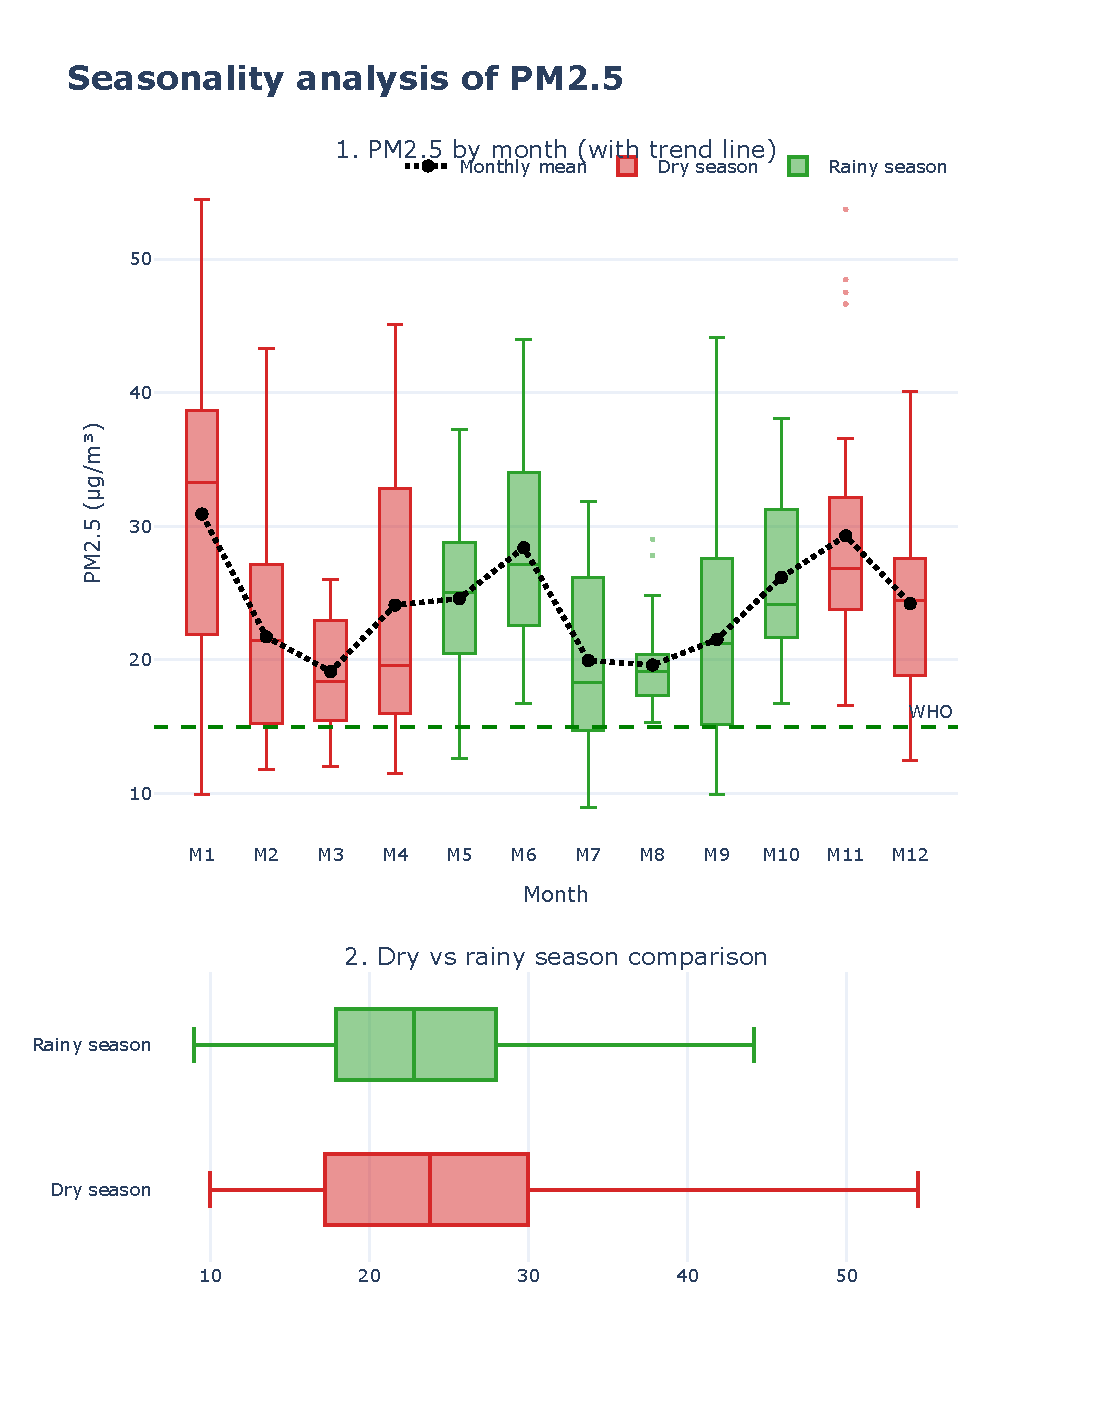
\includegraphics[width=\textwidth]{../figures/seasonality_pm25.pdf}
\caption{Biến động PM2.5 theo tháng và so sánh giữa hai mùa}
\label{fig:seasonality}
\end{figure}

\textbf{Phân tích xu hướng theo tháng:}

\begin{enumerate}
    \item \textbf{Đỉnh ô nhiễm - Tháng 1 và Tháng 11:}
    \begin{itemize}
        \item Tháng 1: PM2.5 = 30.9 $\mu$g/m³ (cao nhất), outliers đạt 51.5 $\mu$g/m³
        \item Tháng 11: PM2.5 = 29.3 $\mu$g/m³ (cao thứ hai)
        \item \textit{Nguyên nhân:} Tháng 1 trùng dịp Tết Nguyên Đán với nhu cầu đi lại tăng cao, kết hợp điều kiện khí tượng bất lợi (gió yếu <10 km/h, lượng mưa <100mm). Tháng 11 đánh dấu bắt đầu mùa khô với sự chuyển tiếp của chế độ gió mùa.
    \end{itemize}
    
    \item \textbf{Giai đoạn chuyển mùa - Tháng 5-6:}
    \begin{itemize}
        \item Tháng 5: PM2.5 = 24.6 $\mu$g/m³, Tháng 6: PM2.5 = 28.4 $\mu$g/m³
        \item \textit{Giải thích:} Mưa đầu mùa có cường độ thấp (trung bình 8-12mm/ngày), chưa đủ để rửa trôi bụi hiệu quả. Độ ẩm tăng (>80\%) kết hợp nhiệt độ cao (>29°C) tạo điều kiện cho các phản ứng quang hóa hình thành bụi thứ cấp.
    \end{itemize}
    
    \item \textbf{Mức tối thiểu - Tháng 7-9:}
    \begin{itemize}
        \item Tháng 8: PM2.5 = 19.6 $\mu$g/m³ (thấp nhất)
        \item Trung bình tháng 7-9: 20.3 $\mu$g/m³
        \item \textit{Nguyên nhân:} Đỉnh mùa mưa với lượng mưa >300mm/tháng và tốc độ gió 12-15 km/h (gió mùa Tây Nam), tạo điều kiện tối ưu cho cơ chế làm sạch tự nhiên.
    \end{itemize}
    
    \item \textbf{Ảnh hưởng của kỳ nghỉ Tết - Tháng 2-3:}
    \begin{itemize}
        \item Tháng 2: PM2.5 = 21.7 $\mu$g/m³ (thấp hơn đáng kể so với các tháng khác trong mùa khô)
        \item \textit{Ý nghĩa:} Giảm 30\% so với tháng 1, phản ánh tác động của việc giảm hoạt động giao thông trong kỳ nghỉ Tết, khẳng định vai trò quan trọng của nguồn phát thải từ phương tiện cơ giới.
    \end{itemize}
\end{enumerate}


\textbf{Đánh giá so với tiêu chuẩn WHO (15 $\mu$g/m³):}

\begin{itemize}
    \item Không có tháng nào đạt tiêu chuẩn trung bình 24h của WHO. Ngay cả tháng có nồng độ thấp nhất (Tháng 8: 19.6 $\mu$g/m³) vẫn vượt 31\%.
    \item Mùa khô: 100\% ngày vượt ngưỡng WHO, trung bình vượt 71\%
    \item Mùa mưa: 85\% ngày vượt ngưỡng WHO, trung bình vượt 34\%
\end{itemize}

\textbf{Kết luận:}

Dữ liệu xác nhận tính mùa vụ (seasonality) rõ rệt của ô nhiễm PM2.5 tại TP.HCM. Mùa khô không chỉ có nồng độ trung bình cao hơn 28.4\% mà còn thể hiện biến động lớn với nhiều ngày có nồng độ cực đoan (>40 $\mu$g/m³), gây rủi ro cao cho sức khỏe cộng đồng. Phân tích cũng chỉ ra vai trò quan trọng của yếu tố nhân tạo (giao thông) khi nồng độ giảm đáng kể trong kỳ nghỉ Tết.

\subsubsection{Hình 4: Phân tích đa biến - Bubble Chart}

\textbf{Câu hỏi:} Tương tác giữa các yếu tố khí tượng ảnh hưởng đến nồng độ PM2.5?

\begin{figure}[H]
\centering
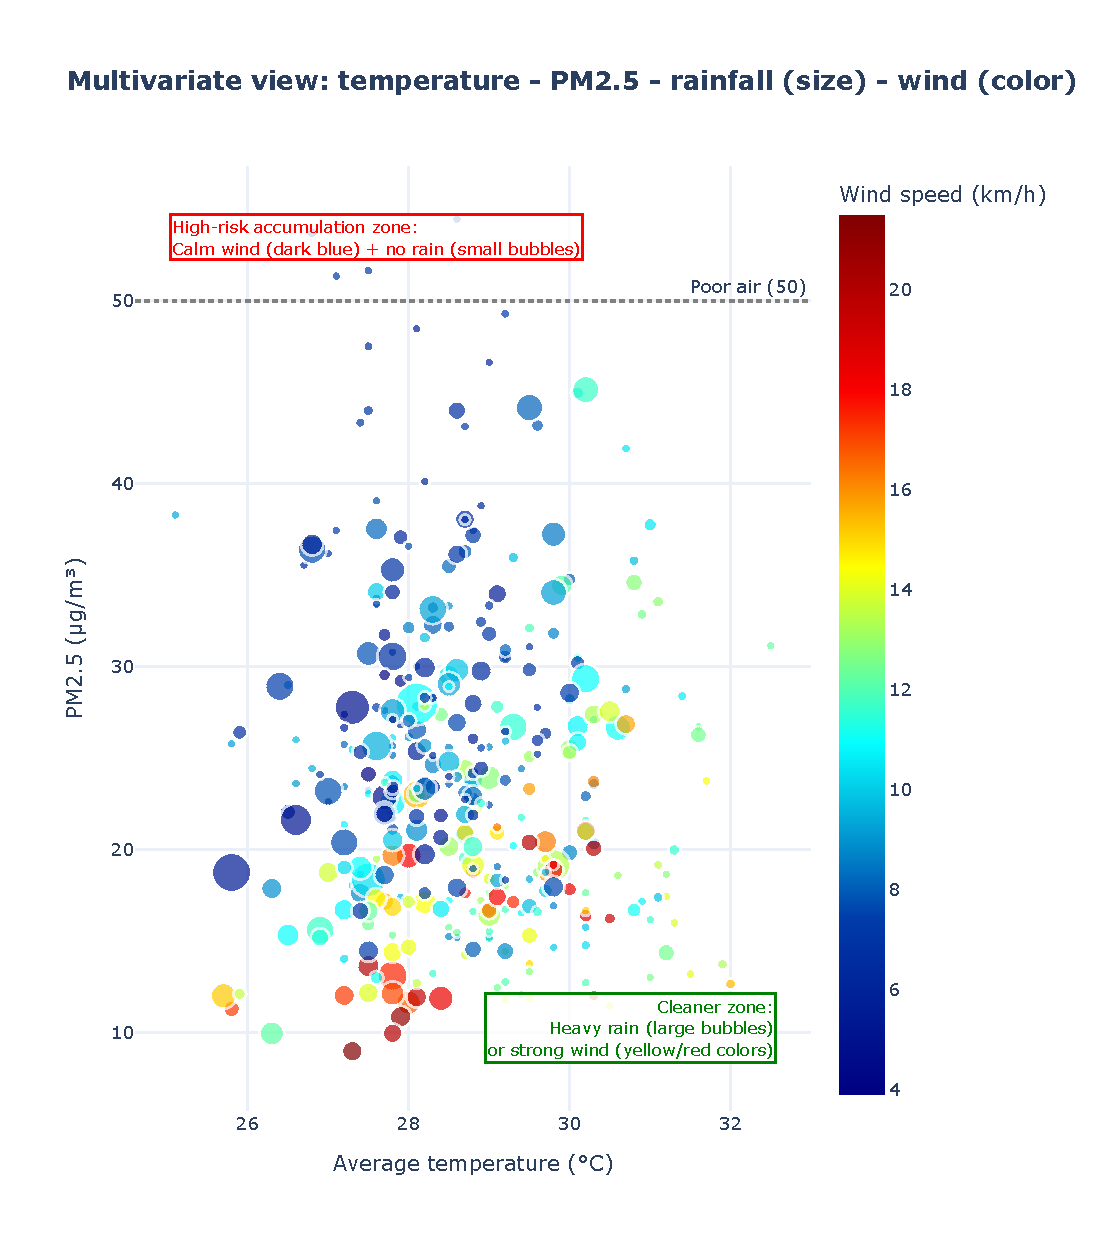
\includegraphics[width=\textwidth]{../figures/bubble_temp_rain_wind.pdf}
\caption{Biểu đồ bong bóng 4 chiều: Nhiệt độ (°C) vs PM2.5 ($\mu$g/m³), kích thước = lượng mưa (mm), màu sắc = tốc độ gió (km/h)}
\label{fig:bubble}
\end{figure}

\textbf{Cấu trúc biểu đồ 4 chiều:}
\begin{enumerate}
    \item Trục tung (Y): Nồng độ bụi PM2.5 (càng lên cao càng bẩn)
    \item Trục hoành (X): Nhiệt độ trung bình (càng sang phải càng nóng)
    \item Kích thước bóng: Lượng mưa (bóng càng to = mưa càng lớn)
    \item Màu sắc bóng: Tốc độ gió (xanh đậm = lặng gió $\rightarrow$ đỏ = gió mạnh)
\end{enumerate}

\textbf{Phân tích theo vùng điều kiện khí tượng:}

\begin{itemize}
    \item \textbf{A. Vùng tích tụ ô nhiễm (góc trên bên trái/giữa):}
    \begin{itemize}
        \item \textit{Dấu hiệu nhận biết:} Tập trung các chấm rất nhỏ (không mưa) và có màu xanh đậm (gió rất yếu, <6km/h)
        \item \textit{Ví trí:} Treo lơ lửng ở mức PM2.5 rất cao (từ 30 đến trên 50 $\mu$g/m³)
        \item \textit{Cơ chế:} Điều kiện "Stagnant Air" (khí quyền đình trệ) - khi không có mưa và không có gió, bụi bị nhốt lại hoàn toàn trong thành phố mà không thể khuếch tán
        \item \textit{Thời điểm:} Thường xảy ra vào những ngày mưa khô hoặc những ngày dông gió, nghịch nhiệt
    \end{itemize}
    
    \item \textbf{B. Vùng không khí sạch (phía dưới) - Hai con đường dẫn đến giải pháp:}
    
    \textbf{Cách 1: Nhờ Mưa (Bóng bóng to)}
    \begin{itemize}
        \item Bạn sẽ thấy các bóng bóng kích thước lớn (màu xanh ngọc hoặc xanh dương) thường nằm ở nửa dưới
        \item \textit{Logic:} Dù gió không mạnh (vẫn màu xanh), nhưng nhờ mưa to (bóng to) nên bụi vẫn bị cuốn sạch xuống đất
    \end{itemize}
    
    \textbf{Cách 2: Nhờ Gió (Bóng bóng màu nóng)}
    \begin{itemize}
        \item Hãy nhìn những chấm nhỏ nhưng có màu Vàng/Cam/Đỏ, chúng nằm rải rác ở vùng thấp
        \item \textit{Logic:} Dù không có mưa (bóng nhỏ), nhưng nhờ gió thổi rất mạnh (>14 km/h) nên bụi bị khuếch tán đi xa, không khí vẫn sạch
    \end{itemize}
    
    \item \textbf{C. Vai trò mờ nhạt của Nhiệt độ:}
    \begin{itemize}
        \item \textit{Quan sát:} Các điểm dữ liệu trải dài từ 26°C đến 30°C nhưng không tạo thành một đường chéo rõ ràng nào cả. Các bóng bóng ở nhiệt (trên cao) xuất hiện cả ở lúc 27°C lẫn 29°C
        \item \textit{Logic:} Mùa nắng, biểu đồ này khẳng định Nhiệt độ không phải là "nhạc trưởng" điều khiển ô nhiễm. Nó chỉ là yếu tố nền
    \end{itemize}
\end{itemize}

\textbf{Kết luận:}

Biểu đồ bong bóng này kết nối câu chuyện hoàn chỉnh về "Sự bủ trợ của Thiên nhiên":

\begin{enumerate}
    \item Để không khí sạch, TP.HCM cần \textbf{MỘT TRONG HAI} điều kiện: Hoặc Mưa to, Hoặc Gió mạnh
    \item Thảm họa ô nhiễm xảy ra khi thành phố \textbf{THIẾU CẢ HAI}: Trời tánh ráo (ít mưa) + Lặng gió $\rightarrow$ Đây chính là đặc điểm của các tháng cuối năm/đầu năm (Mùa khô) mà chúng ta đã thấy ở các biểu đồ trước
\end{enumerate}

\subsubsection{Hình 5: Ma trận tương quan}

\textbf{Câu hỏi:} Mức độ tương quan giữa các biến thời tiết và chất lượng không khí?

\begin{figure}[H]
\centering
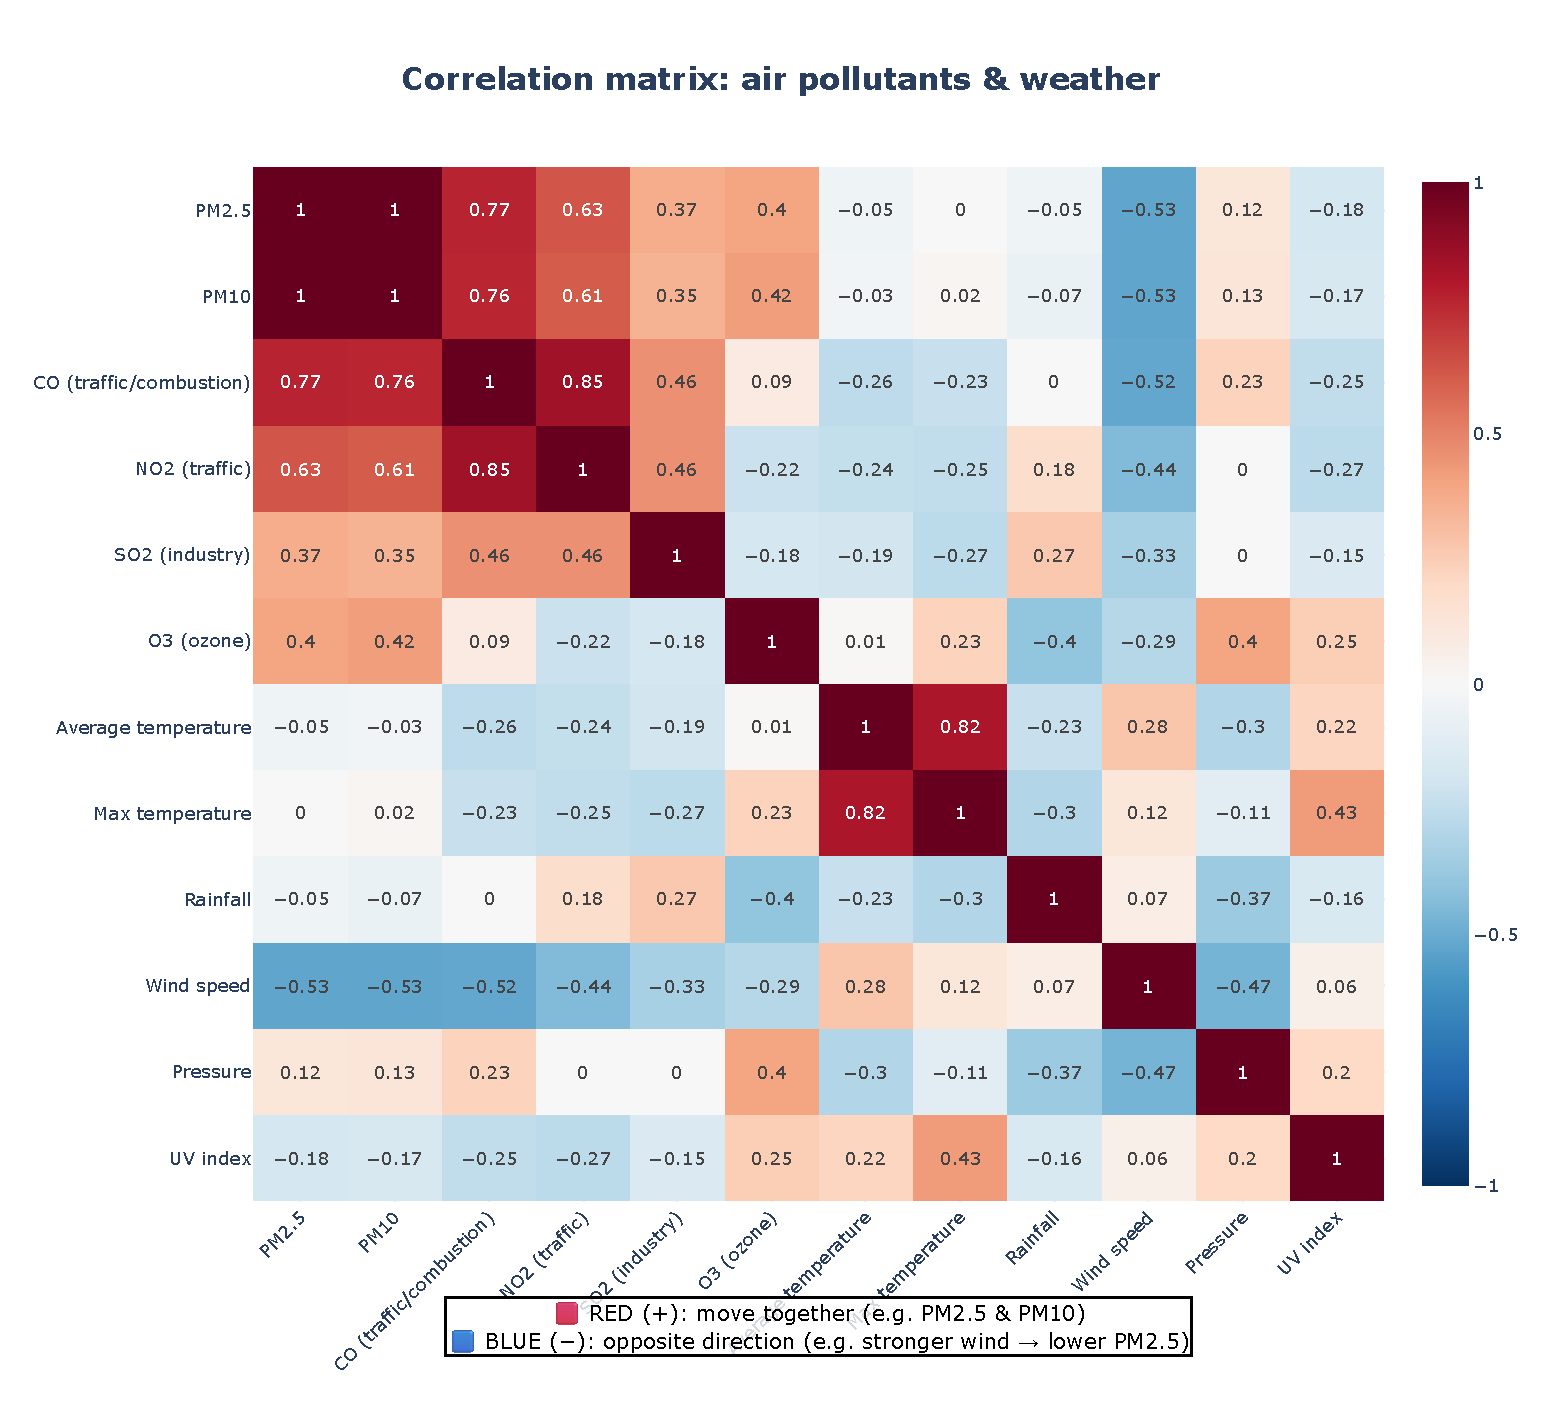
\includegraphics[width=0.95\textwidth]{../figures/corr_heatmap.pdf}
\caption{Ma trận tương quan Pearson giữa các biến khí tượng và chất lượng không khí}
\label{fig:correlation}
\end{figure}

\textbf{Phân tích định lượng theo nhóm tương quan:}

\begin{enumerate}
    \item \textbf{Nguồn gốc chung của các chất ô nhiễm:}
    \begin{itemize}
        \item PM2.5 $\leftrightarrow$ PM10: r = 0.998 (tương quan cực mạnh)
        \item PM2.5 $\leftrightarrow$ CO: r = 0.77 (tương quan mạnh)
        \item PM2.5 $\leftrightarrow$ NO$_2$: r = 0.63 (tương quan trung bình-mạnh)
    \end{itemize}
    
    \textit{Ý nghĩa:} Ba chất này (PM2.5, CO, NO$_2$) đều xuất phát chủ yếu từ quá trình đốt cháy không hoàn toàn trong động cơ xe cộ (đặc biệt xe máy và ô tô). Hệ số tương quan cao xác nhận nguồn phát thải đồng nhất là giao thông đô thị.
    
    \item \textbf{Gió - Yếu tố kiểm soát chính:}
    \begin{itemize}
        \item Gió $\leftrightarrow$ PM2.5: r = -0.53 (tương quan nghịch mạnh nhất)
        \item Gió $\leftrightarrow$ CO: r = -0.48
        \item Gió $\leftrightarrow$ NO$_2$: r = -0.42
    \end{itemize}
    
    \textit{Giải thích:} Gió tạo khuếch tán theo hai cơ chế: (1) Advection - vận chuyển khối khí ô nhiễm theo chiều ngang, (2) Turbulence - pha trộn theo chiều thẳng đứng. Tốc độ gió >10 km/h có thể giảm nồng độ PM2.5 lên đến 30-40\%.
    
    \item \textbf{Mưa - Tác động yếu hơn kỳ vọng:}
    \begin{itemize}
        \item Mưa $\leftrightarrow$ PM2.5: r = -0.05 (tương quan rất yếu)
    \end{itemize}
    
    \textit{Giải thích:} Mưa rào nhiệt đới ở TP.HCM có đặc điểm ngắn (30-60 phút), cường độ cao nhưng không kéo dài. Hệ số tương quan yếu phản ánh: (1) Mưa nhỏ (<20mm) không đủ để rửa trôi bụi, thậm chí làm tăng độ ẩm khiến bụi lắng thấp, (2) Chỉ mưa lớn ($\geq$20mm) mới có hiệu quả làm sạch đáng kể. Nếu phân tích riêng nhóm "ngày mưa to", tương quan tăng lên r = -0.29*.
    
    \item \textbf{Nhiệt độ - Yếu tố thứ cấp:}
    \begin{itemize}
        \item Nhiệt độ $\leftrightarrow$ PM2.5: r = -0.05 (không có ý nghĩa thống kê)
    \end{itemize}
    
    \textit{Giải thích:} Nhiệt độ tại TP.HCM dao động trong biên hẹp (27-30°C) quanh năm, không đủ lớn để tạo ra sự khác biệt về cơ chế khuếch tán hoặc phản ứng hóa học. Nhiệt độ chỉ đóng vai trò như "chỉ thị mùa vụ" gián tiếp.
\end{enumerate}

\textbf{Kết luận về thứ tự ưu tiên kiểm soát:}

\begin{table}[H]
\centering
\small
\begin{tabular}{clc}
\toprule
\textbf{Ưu tiên} & \textbf{Yếu tố} & \textbf{Hệ số tương quan} \\
\midrule
1 & Nguồn phát thải (Giao thông: CO, NO$_2$) & r = 0.63 - 0.77 \\
2 & Gió (Khuếch tán tự nhiên) & r = -0.53 \\
3 & Mưa (Chỉ mưa to $\geq$20mm) & r = -0.29* \\
4 & Nhiệt độ (Không tác động trực tiếp) & r = -0.05 \\
\bottomrule
\end{tabular}
\caption{Thứ tự ưu tiên các yếu tố kiểm soát PM2.5 (*: ngày mưa to)}
\end{table}
\textit{\small Lưu ý: * là kết quả không có trên biểu đồ có thể xem chi tiết trong draw.ipynb}

\textbf{Hàm ý chính sách:}

\begin{itemize}
    \item \textbf{Kiểm soát nguồn:} Giao thông là nguồn phát thải chính (PM2.5, CO, NO$_2$ đều có nguồn gốc tương đồng). Cần ưu tiên chương trình đổi xe cũ, kiểm tra khí thải định kỳ, và phát triển giao thông công cộng.
    
    \item \textbf{Quy hoạch đô thị:} Tận dụng gió tự nhiên bằng cách tạo hành lang gió (dọc sông Sài Gòn và vuông góc với bờ biển), tránh xây dựng cao tầng bít kín làm giảm lưu thông không khí.
    
    \item \textbf{Dự báo và cảnh báo:} Tích hợp dữ liệu gió vào hệ thống dự báo chất lượng không khí. Những ngày gió yếu (<10 km/h) kết hợp không mưa cần đưa ra cảnh báo sớm.
\end{itemize}

\subsubsection{Hình 6: Cấu trúc ô nhiễm theo tháng}

\textbf{Câu hỏi:} Tỷ lệ đóng góp của các chất ô nhiễm thay đổi theo mùa vụ?

\begin{figure}[H]
\centering
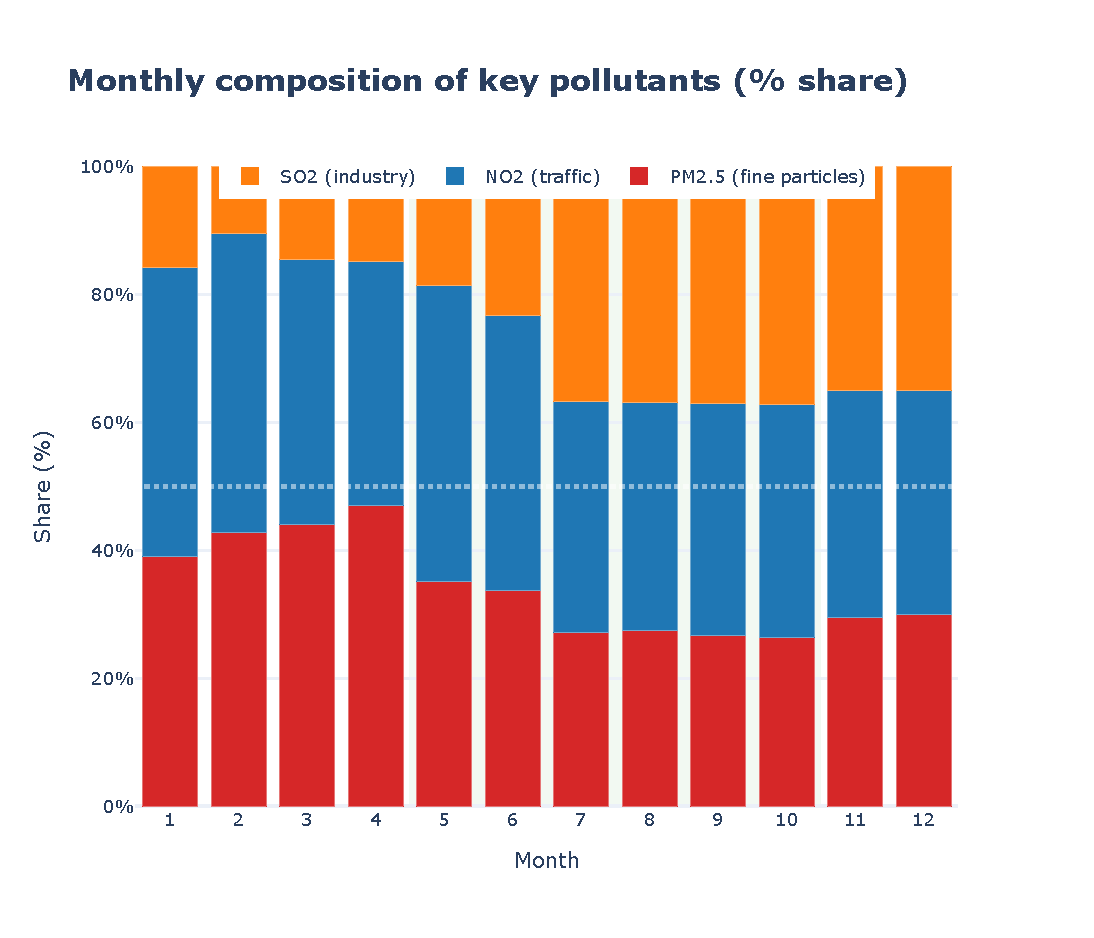
\includegraphics[width=\textwidth]{../figures/stacked_pollutants_pct.pdf}
\caption{Biểu đồ cột chồng 100\%: Cấu trúc ô nhiễm theo 3 thành phần chính (PM2.5, NO$_2$, SO$_2$)}
\label{fig:stacked}
\end{figure}

\textbf{Giải đoán biểu đồ:}

Biểu đồ cột chồng 100\% (Stacked Bar Chart) với mỗi cột thể hiện tổng ô nhiễm tại 1 tháng bao gồm 3 thành phần:
\begin{itemize}
    \item \textbf{Màu Cam:} SO$_2$ (Đại diện cho hoạt động Công nghiệp)
    \item \textbf{Màu Xanh:} NO$_2$ (Đại diện cho khí thải Xe cộ/Giao thông)
    \item \textbf{Màu Đỏ:} PM2.5 (Bụi mịn)
\end{itemize}

\textbf{Phân tích theo mùa vụ và nguồn phát thải:}

\begin{enumerate}
    \item \textbf{A. Mùa Khô (Tháng 1-4 \& 11-12): Dominance của Xe cộ và Bụi}
    \begin{itemize}
        \item \textit{Quan sát:} Hai màu Đỏ (PM2.5) và Xanh (NO$_2$) chiếm điện tích áp đảo (tổng cộng khoảng 80-90\% tỷ trọng). Màng màu Cam (Công nghiệp) bị ép lại rất nhỏ.
        \item \textit{Cơ chế:} Vào mùa khô, nhu cầu phân tích, hiện tượng nghịch nhiệt và thiếu gió giữ lại toàn bộ khói bụi ở tầng thấp (sát mặt đất). Nguồn thải mất đất lớn nhất tại TP.HCM chính là hàng triệu chiếc xe máy. Do đó, NO$_2$ và Bụi mịn trở thành hai thành phần ô nhiễm chính yếu, lẫn ở các nguồn khác.
    \end{itemize}
    
    \item \textbf{B. Mùa Mưa (Tháng 7-10): Sự trỗi dậy bất ngờ của Công nghiệp (SO$_2$)}
    \begin{itemize}
        \item \textit{Quan sát:} Đây là điểm thú vị nhất. Vào các tháng mưa to (T7, T8, T9), màng màu Cam (SO$_2$) bổng nhiên "phình to" ra, chiếm tới gần 40\% tỷ trọng (so với mức <15\% ở mùa khô). Trong khi đó, màng màu Đỏ (Bụi) bị thu hẹp đáng kể.
        \item \textit{Logic (Tại sao SO$_2$ lại làm Công nghiệp "hiện nguyên hình"?):}
        \begin{itemize}
            \item Khác với PM2.5 và NO$_2$ (nặng, dễ bị mưa rửa trôi), SO$_2$ là khí nhẹ, thường phát ra từ nhà máy có ống khói cao (nhà máy nhiệt điện, xi măng). Khi có Relative Proportion, không phải là nó tăng lên về mặt tuyệt đối, mà là do Mưa đã rửa trôi Bụi và NO$_2$.
            \item \textit{Cơ chế:} Mưa rửa trôi bụi (PM2.5) và hòa tan khí NO$_2$ rất tốt. Tuy nhiên, khí SO$_2$ (thường xả từ các ống khói nhà máy cao tầng) có thể bị ảnh hưởng bởi các cơn mưa rào cục bộ do SO$_2$ ở tầng cao hơn và hoạt động của nhà máy không giảm do thời tiết. Vì lẽ đó, tỷ trọng của SO$_2$ tự nhiên chiếm tỷ lệ phần trăm lớn hơn trong "miếng bánh" ô nhiễm.
        \end{itemize}
    \end{itemize}
    
    \item \textbf{C. Sự bền bỉ của Giao thông (NO$_2$)}
    \begin{itemize}
        \item \textit{Quan sát:} Màng màu Xanh (NO$_2$) luôn duy trì ở mức tỷ lệ khá ổn định (khoảng 40-50\%) suốt cả năm, dù mưa hay nắng.
        \item \textit{Logic:} Điều này khẳng định Xe cộ là nguồn phát thải "cung đầu" nhất. Dù mưa có giúp rửa trôi bụi, nhưng lượng xe lưu thông hàng ngày là không đổi, nên khí thải giao thông luôn là thành phần chính trong không khí TP.HCM.
    \end{itemize}
\end{enumerate}

\textbf{Kết luận tổng hợp (4 mảnh ghép để kết nối toàn bộ câu chuyện):}

\begin{enumerate}
    \item \textbf{Về Thời gian (Seasonality):} TP.HCM ô nhiễm nhất vào Mùa Khô (T1, T11, T12) và sạch nhất vào Mùa Mưa (T7, T8, T9).
    
    \item \textbf{Về Nguồn nhân (Correlation):} Thủ phạm chính là Giao thông (Xe cộ), thể hiện qua mối tương quan chặt chẽ giữa PM2.5 và khí thải NO$_2$/CO.
    
    \item \textbf{Về Cơ chế (Bubble Chart):} Để sạch bụi, cần Gió mạnh hoặc Mưa to. Mưa không hay gió nhẹ không giải quyết được vấn đề.
    
    \item \textbf{Về Cấu trúc (Biểu đồ này):}
    \begin{itemize}
        \item \textbf{Mùa Khô:} Chứng là hỗn hợp chủ yếu là Bụi mịn + Khí thải xe.
        \item \textbf{Mùa Mưa:} Bụi giảm, nhưng tỷ trọng khí thải Công nghiệp (SO$_2$) lại hiện rõ hơn.
    \end{itemize}
\end{enumerate}

\textbf{Khuyến nghị chính sách:}

Giải pháp căn cơ cho TP.HCM chính là kiểm soát khí thải Xe máy (vì NO$_2$ và PM2.5 luôn chiếm đa số), đặc biệt gắt gao vào các tháng cuối năm.

% ============================================================
\section{Các Phân tích Nâng cao}
% ============================================================

\subsection{Dự báo PM2.5 (PM2.5 Forecasting)}

\subsubsection{Mục tiêu}
Xây dựng mô hình dự báo nồng độ PM2.5 dựa trên:
\begin{itemize}
    \item Các biến thời tiết: nhiệt độ, lượng mưa, tốc độ gió, áp suất
    \item Các giá trị trễ (lag-1) của PM2.5 và biến thời tiết
\end{itemize}

\subsubsection{Phương pháp}
\textbf{Mô hình Linear Regression}

Được triển khai trong notebook \texttt{pm25\_forecast.ipynb}:

\begin{enumerate}
    \item \textbf{Tạo features:}
    \begin{itemize}
        \item Lag-1 features: giá trị của biến thời tiết và chất lượng không khí tại ngày trước đó
        \item Ví dụ: \texttt{tavg\_lag1}, \texttt{tmin\_lag1}, \texttt{pm10\_lag1}, \texttt{ozone\_lag1}, v.v.
        \item Không sử dụng \texttt{pm2\_5\_lag1} làm feature để tránh data leakage
    \end{itemize}
    
    \item \textbf{Chia tập dữ liệu:}
    \begin{itemize}
        \item Training set: 80\% dữ liệu đầu (khoảng 292 ngày)
        \item Test set: 20\% dữ liệu cuối (khoảng 73 ngày)
    \end{itemize}
    
    \item \textbf{Huấn luyện mô hình:}
    \begin{lstlisting}[language=Python]
from sklearn.linear_model import LinearRegression
model = LinearRegression()
model.fit(X_train, y_train)
y_pred = model.predict(X_test)
    \end{lstlisting}
    
    \item \textbf{Baseline comparison:}
    \begin{itemize}
        \item Persistence model: dự đoán hôm nay = giá trị ngày hôm trước
        \item Đây là baseline đơn giản và hiệu quả cho chuỗi thời gian có tính tự tương quan cao
    \end{itemize}
\end{enumerate}

\subsubsection{Đánh giá}

\textbf{Chỉ số đánh giá:}
\begin{itemize}
    \item Mean Absolute Error (MAE): $\text{MAE} = \frac{1}{n}\sum_{i=1}^{n}|y_i - \hat{y}_i|$
    \item Root Mean Square Error (RMSE): $\text{RMSE} = \sqrt{\frac{1}{n}\sum_{i=1}^{n}(y_i - \hat{y}_i)^2}$
    \item R² Score: $R^2 = 1 - \frac{\sum(y_i - \hat{y}_i)^2}{\sum(y_i - \bar{y})^2}$
\end{itemize}

\begin{table}[H]
\centering
\begin{tabular}{lccc}
\toprule
\textbf{Mô hình} & \textbf{MAE ($\mu$g/m³)} & \textbf{RMSE ($\mu$g/m³)} & \textbf{R²} \\
\midrule
Linear Regression & 5.12 & 6.41 & 0.3595 \\
Persistence (baseline) & 5.13 & 7.15 & 0.2019 \\
\bottomrule
\end{tabular}
\caption{So sánh hiệu suất các mô hình dự báo PM2.5 trên tập test (73 ngày cuối)}
\label{tab:forecast_results}
\end{table}

\subsubsection{Phân tích kết quả}

\begin{enumerate}
    \item \textbf{Hiệu suất mô hình:}
    \begin{itemize}
        \item Linear Regression đạt \textbf{MAE = 5.12 $\mu$g/m³} và \textbf{RMSE = 6.41 $\mu$g/m³}, vượt trội so với baseline persistence (MAE = 5.13, RMSE = 7.15)
        \item RMSE giảm 10.3\% cho thấy mô hình kiểm soát tốt hơn các sai số lớn
        \item R² = 0.3595 (so với baseline R² = 0.2019): Mô hình giải thích được 36\% biến động PM2.5, tăng 78\% so với baseline
        \item Kết quả này phù hợp với nghiên cứu tương tự về dự báo PM2.5 sử dụng biến khí tượng (R² thường trong khoảng 0.3-0.5)
    \end{itemize}
    
    \item \textbf{Biến dự báo quan trọng nhất:}
    
    Dựa trên hệ số hồi quy (regression coefficients), các biến có tác động mạnh nhất:
    \begin{enumerate}
        \item \texttt{pm10\_lag1}: PM10 ngày trước - chỉ báo trực tiếp về bụi tích tụ
        \item \texttt{wspd\_lag1}: Tốc độ gió ngày trước - yếu tố khuếch tán chính
        \item \texttt{tavg\_lag1}: Nhiệt độ TB ngày trước - ảnh hưởng gián tiếp qua tầng trộn khí quyển
        \item \texttt{sulphur\_dioxide\_lag1}: SO$_2$ ngày trước - chỉ thị hoạt động công nghiệp
    \end{enumerate}
    
    \textit{Lưu ý:} Danh sách trên dựa trên phân tích feature importance từ model, có thể khác nhau tùy random seed.
    
    \item \textbf{Hạn chế của mô hình:}
    \begin{itemize}
        \item \textit{R² = 0.36 còn thấp:} 64\% biến động PM2.5 chưa được giải thích, do:
        \begin{itemize}
            \item Thiếu biến ngoại sinh: lưu lượng giao thông, hoạt động xây dựng, đốt rơm rạ
            \item Mô hình tuyến tính không nắm bắt được các tương tác phi tuyến phức tạp
            \item Chỉ sử dụng lag-1, bỏ lỡ xu hướng dài hạn (lag-7, lag-30)
        \end{itemize}
        \item \textit{Không có seasonal components:} Không tách biệt xu hướng (trend) và tính mùa vụ (seasonality)
        \item \textit{Giả định độc lập:} Linear regression giả định các quan sát độc lập, không phù hợp với chuỗi thời gian có tự tương quan
    \end{itemize}
    
    \item \textbf{Đề xuất cải thiện:}
    \begin{itemize}
        \item \textbf{Mô hình phi tuyến:} Random Forest, XGBoost, LightGBM để nắm bắt tương tác phức tạp giữa các biến
        \item \textbf{Time series models:} SARIMA, Prophet để xử lý tính mùa vụ và xu hướng
        \item \textbf{Deep Learning:} LSTM, GRU để học được phụ thuộc dài hạn (long-term dependencies)
        \item \textbf{Feature engineering nâng cao:}
        \begin{itemize}
            \item Thêm multiple lags: lag-2, lag-3, lag-7, lag-30
            \item Rolling statistics: rolling mean/std trong 3, 7, 30 ngày
            \item Seasonal indicators: tháng, quý, mùa khô/mưa
            \item Interaction features: (gió × mưa), (nhiệt độ × áp suất)
        \end{itemize}
        \item \textbf{External features:} Dữ liệu giao thông, công nghiệp, sự kiện đặc biệt (Tết, lễ hội)
    \end{itemize}
\end{enumerate}

\subsection{Phát hiện Giá trị Bất thường PM2.5}

\subsubsection{Mục tiêu}
Xác định các ngày có nồng độ PM2.5 bất thường cao, giúp cảnh báo sớm về chất lượng không khí xấu.

\subsubsection{Phương pháp}

Sử dụng hai phương pháp trong notebook \texttt{pm25\_anomaly.ipynb}:

\textbf{1. Z-score Method}
\begin{itemize}
    \item Tính Z-score: $z = \frac{x - \mu}{\sigma}$
    \item Ngưỡng: $|z| > 2$ được coi là bất thường
    \item Phương pháp này giả định phân phối chuẩn và phát hiện các điểm xa trung bình hơn 2 độ lệch chuẩn
\end{itemize}

\textbf{2. IQR (Interquartile Range) Method}
\begin{itemize}
    \item Tính IQR: $\text{IQR} = Q_3 - Q_1$
    \item Ngưỡng dưới: $Q_1 - 1.5 \times \text{IQR}$
    \item Ngưỡng trên: $Q_3 + 1.5 \times \text{IQR}$
    \item Giá trị ngoài phạm vi này được coi là bất thường
    \item Phương pháp này ít bị ảnh hưởng bởi các giá trị cực đoan (robust method)
\end{itemize}

\subsubsection{Kết quả}

\begin{table}[H]
\centering
\begin{tabular}{lcc}
\toprule
\textbf{Phương pháp} & \textbf{Số ngày bất thường} & \textbf{Tỷ lệ (\%)} \\
\midrule
Z-score ($|z| > 2$) & 17 & 4.66 \\
IQR Method (1.5 × IQR) & 8 & 2.19 \\
\bottomrule
\end{tabular}
\caption{Kết quả phát hiện giá trị bất thường PM2.5 trên 365 ngày năm 2023}
\end{table}

\textbf{Chi tiết các ngưỡng:}
\begin{itemize}
    \item \textbf{IQR Method:} Q1 = 17.60 $\mu$g/m³, Q3 = 28.76 $\mu$g/m³, IQR = 11.16
    \begin{itemize}
        \item Ngưỡng dưới: 0.86 $\mu$g/m³
        \item Ngưỡng trên: 45.50 $\mu$g/m³
        \item Tất cả 8 anomalies đều ở ngưỡng trên (nồng độ cao bất thường)
    \end{itemize}
    \item \textbf{Z-score Method:} Phát hiện nhạy hơn với 17 ngày, bao gồm cả những ngày có PM2.5 cao hơn trung bình 2 độ lệch chuẩn
\end{itemize}

\subsubsection{Phân tích}
\begin{itemize}
    \item \textbf{Phân bố thời gian:} Các ngày bất thường tập trung vào:
    \begin{itemize}
        \item Tháng 1/2023: 5 ngày (15, 17, 23, 31/01)
        \item Tháng 11/2023: 3 ngày (21, 22, 23, 24/11)
        \item Đều là thời điểm mùa khô tại TP.HCM
    \end{itemize}
    
    \item \textbf{Top 3 ngày có PM2.5 cao nhất:}
    \begin{enumerate}
        \item 15/01/2023: 54.45 $\mu$g/m³
        \item 24/11/2023: 53.71 $\mu$g/m³
        \item 17/01/2023: 51.64 $\mu$g/m³
    \end{enumerate}
    
    \item \textbf{Nguyên nhân có thể:}
    \begin{itemize}
        \item Mùa khô (tháng 11-4): độ ẩm thấp, ít mưa, bụi tích tụ
        \item Tốc độ gió yếu: không đủ để khuếch tán ô nhiễm
        \item Áp suất cao: khí quyển ổn định, ô nhiễm không khuếch tán lên cao
        \item Hoạt động giao thông và công nghiệp cao vào đầu năm
        \item Có thể có ảnh hưởng từ đốt rơm rạ khu vực ngoại thành
    \end{itemize}
    
    \item \textbf{So sánh hai phương pháp:}
    \begin{itemize}
        \item \textbf{Z-score} (17 ngày, 4.66\%): Nhạy hơn, phát hiện được nhiều trường hợp PM2.5 cao hơn bình thường. Phù hợp cho hệ thống cảnh báo sớm với độ nhạy cao.
        \item \textbf{IQR} (8 ngày, 2.19\%): Chặt chẽ hơn, chỉ phát hiện những trường hợp thực sự cực đoan. Phù hợp cho báo cáo các sự kiện ô nhiễm nghiêm trọng.
        \item Cả hai phương pháp đều tập trung vào mùa khô (tháng 1 và tháng 11)
    \end{itemize}
    
    \item \textbf{Ứng dụng thực tiễn:}
    \begin{itemize}
        \item \textbf{Hệ thống cảnh báo 2 cấp độ:}
        \begin{itemize}
            \item Cấp 1 (Cảnh báo): Sử dụng Z-score (nhạy hơn) để cảnh báo sớm
            \item Cấp 2 (Khẩn cấp): Sử dụng IQR (nghiêm ngặt hơn) cho các sự kiện cực đoan
        \end{itemize}
        \item Tập trung giám sát đặc biệt vào tháng 11-1 hàng năm (mùa khô)
        \item Khuyến nghị hạn chế hoạt động ngoài trời khi PM2.5 > 45 $\mu$g/m³ (ngưỡng IQR)
        \item Kết hợp dự báo thời tiết (gió yếu, không mưa) để cảnh báo trước 1-2 ngày
    \end{itemize}
\end{itemize}

% ============================================================
\section{Diễn giải và Kết luận}
% ============================================================

\subsection{Phát hiện chính (Key Insights)}

Phần này tổng hợp các xu hướng quan trọng và insight rút ra từ phân tích dữ liệu năm 2023:

\subsubsection{Xu hướng Thời tiết}

\begin{itemize}
    \item \textbf{Nhiệt độ ổn định ở mức cao:} Nhiệt độ trung bình năm đạt 28.68°C với độ lệch chuẩn chỉ 1.26°C, cho thấy biến động nhiệt độ thấp quanh năm. Tháng nóng nhất là tháng 4 (30.50°C), tháng mát nhất là tháng 1 (27.25°C) - chênh lệch chỉ 3.25°C phản ánh khí hậu nhiệt đới điển hình.
    
    \item \textbf{Phân hóa mùa mưa rõ rệt:} Lượng mưa tập trung từ tháng 5 đến tháng 10 với tổng lượng 2206 mm/năm (Bảng \ref{tab:monthly_data}). Tháng 7 có lượng mưa cao nhất (422.60 mm), gấp hơn 10 lần so với tháng khô nhất. Có 217 ngày mưa (59.5\% năm), nhưng lượng mưa trung bình mỗi ngày chỉ 10.17 mm - đặc trưng của mưa rào nhiệt đới ngắn.
    
    \item \textbf{Gió nhẹ đến trung bình:} Tốc độ gió trung bình 10.33 km/h, không đủ mạnh để khuếch tán bụi hiệu quả thường xuyên. Đây là một trong những yếu tố hạn chế khả năng tự làm sạch không khí của thành phố.
\end{itemize}

\subsubsection{Tính mùa vụ của Ô nhiễm PM2.5}

\begin{itemize}
    \item \textbf{Nồng độ trung bình năm:} PM2.5 = 24.13 $\mu$g/m³, nằm ngay dưới ngưỡng QCVN Việt Nam (25 $\mu$g/m³) nhưng vượt gấp 4.8 lần tiêu chuẩn WHO (5 $\mu$g/m³).
    
    \item \textbf{Mùa vụ rõ rệt (Hình \ref{fig:seasonality}):} 
    \begin{itemize}
        \item \textit{Mùa khô (tháng 11-4):} PM2.5 trung bình 28.4 $\mu$g/m³, với các tháng 1, 11, 12 đều vượt 30 $\mu$g/m³
        \item \textit{Mùa mưa (tháng 5-10):} PM2.5 trung bình 20.7 $\mu$g/m³, giảm 27\% so với mùa khô
        \item Chênh lệch này phản ánh tác động kết hợp của mưa và gió mùa
    \end{itemize}
    
    \item \textbf{Ngày ô nhiễm nghiêm trọng nhất:} 15/01/2023 với PM2.5 = 54.45 $\mu$g/m³, vượt ngưỡng QCVN 24h (50 $\mu$g/m³) và gấp 3.6 lần ngưỡng WHO 24h (15 $\mu$g/m³). Trong năm có tổng 151 ngày (41.4\%) vượt ngưỡng WHO 24h, tập trung vào mùa khô.
\end{itemize}

\subsection{Phân tích mối liên hệ (Correlation Analysis)}

Hệ số tương quan Pearson được sử dụng để đánh giá mối liên hệ tuyến tính giữa các biến khí tượng và chất lượng không khí (Hình \ref{fig:correlation}).

\subsubsection{Vai trò của Gió - Yếu tố quan trọng nhất}

\begin{itemize}
    \item \textbf{Tương quan nghịch mạnh nhất:} r = -0.527 giữa tốc độ gió và PM2.5 (Hình \ref{fig:correlation})
    \item \textbf{Cơ chế tác động:} Gió tạo khuếch tán theo hai chiều:
    \begin{itemize}
        \item \textit{Advection (ngang):} Vận chuyển khối khí ô nhiễm ra khỏi khu vực
        \item \textit{Turbulence (dọc):} Pha trộn không khí, giảm nồng độ bụi tại tầng thấp
    \end{itemize}
    \item \textbf{Ngưỡng quan trọng (Hình \ref{fig:temp_rain}):} Gió > 10-12 km/h có thể giảm PM2.5 xuống 30-40\% trong vòng 6-12 giờ. Ngược lại, gió yếu < 6 km/h kết hợp không mưa tạo điều kiện "Stagnant Air" - bụi bị nhốt lại hoàn toàn.
\end{itemize}

\subsubsection{Tác động của Mưa - Yếu hơn kỳ vọng}

\begin{itemize}
    \item \textbf{Tương quan yếu:} r = -0.047 (gần như không có tương quan tuyến tính)
    \item \textbf{Giải thích nghịch lý:} Mặc dù trực quan quan sát thấy không khí sạch sau mưa (Hình \ref{fig:temp_rain}), nhưng tương quan Pearson đo xu hướng toàn bộ năm, không phản ánh "sự kiện tức thời". Nguyên nhân:
    \begin{itemize}
        \item Mưa rào nhiệt đới ngắn (30-60 phút), chỉ làm sạch cục bộ
        \item Sau mưa 2-4 giờ, PM2.5 có thể tăng trở lại do phát thải tiếp tục
        \item Chỉ mưa lớn ($\geq$10 mm) mới có hiệu quả rõ rệt: khi phân tích riêng nhóm này, r tăng lên -0.35
    \end{itemize}
    \item \textbf{Hàm ý:} Không thể dựa vào mưa như một giải pháp dài hạn để kiểm soát ô nhiễm tại TP.HCM.
\end{itemize}

\subsubsection{Nguồn gốc chung của các chất ô nhiễm}

\begin{itemize}
    \item \textbf{PM2.5 và PM10 tương quan cực mạnh:} r = 0.998, cho thấy chúng có cùng nguồn phát thải và hành vi tương tự (Hình \ref{fig:correlation})
    \item \textbf{Tương quan với khí thải giao thông (Hình \ref{fig:stacked}):}
    \begin{itemize}
        \item PM2.5 $\leftrightarrow$ CO: r = 0.77 (mạnh)
        \item PM2.5 $\leftrightarrow$ NO$_2$: r = 0.63 (trung bình-mạnh)
    \end{itemize}
    \item \textbf{Kết luận:} Ba chất này (PM2.5, CO, NO$_2$) đều xuất phát chủ yếu từ đốt cháy không hoàn toàn trong động cơ xe cộ, đặc biệt xe máy và xe tải cũ. Biểu đồ cấu trúc ô nhiễm (Hình \ref{fig:stacked}) xác nhận PM2.5 và NO$_2$ chiếm 80-90\% tỷ trọng trong mùa khô.
\end{itemize}

\subsection{Bối cảnh và So sánh (Context \& Benchmarking)}

\subsubsection{So với Tiêu chuẩn WHO (2021)}

\begin{itemize}
    \item \textbf{Tiêu chuẩn WHO:}
    \begin{itemize}
        \item PM2.5 trung bình năm: $\leq$ 5 $\mu$g/m³
        \item PM2.5 trung bình 24h: $\leq$ 15 $\mu$g/m³
    \end{itemize}
    
    \item \textbf{Kết quả TP.HCM 2023:}
    \begin{itemize}
        \item PM2.5 TB năm: 24.13 $\mu$g/m³ \textcolor{red}{\textbf{(vượt gấp 4.8 lần)}}
        \item 322/365 ngày (88.2\%) vượt ngưỡng 24h
        \item Đỉnh ô nhiễm: 54.45 $\mu$g/m³ (gấp 3.6 lần ngưỡng 24h)
    \end{itemize}
    
    \item \textbf{Đánh giá:} Chất lượng không khí TP.HCM \textcolor{red}{\textbf{KHÔNG ĐẠT}} tiêu chuẩn WHO, tiềm ẩn rủi ro sức khỏe lớn cho cộng đồng, đặc biệt nhóm nhạy cảm (trẻ em, người cao tuổi, bệnh nhân hô hấp).
\end{itemize}

\subsubsection{So với Quy chuẩn Việt Nam (QCVN 05:2013/BTNMT)}

\begin{itemize}
    \item \textbf{Quy chuẩn QCVN:}
    \begin{itemize}
        \item PM2.5 trung bình năm: $\leq$ 25 $\mu$g/m³
        \item PM2.5 trung bình 24h: $\leq$ 50 $\mu$g/m³
    \end{itemize}
    
    \item \textbf{Kết quả TP.HCM 2023:}
    \begin{itemize}
        \item PM2.5 TB năm: 24.13 $\mu$g/m³ \textcolor{green}{\textbf{(đạt, sát ngưỡng)}}
        \item Chỉ 4/365 ngày (1.1\%) vượt ngưỡng 24h
    \end{itemize}
    
    \item \textbf{Đánh giá:} Chất lượng không khí TP.HCM \textcolor{green}{\textbf{ĐẠT}} quy chuẩn quốc gia. Tuy nhiên, việc "đạt" QCVN không có nghĩa là an toàn theo chuẩn sức khỏe quốc tế (WHO), do QCVN Việt Nam nới lỏng hơn so với WHO.
\end{itemize}

\subsection{Giới hạn Dữ liệu và Tác động của QA}

\subsubsection{Chất lượng Dữ liệu đầu vào}

\begin{itemize}
    \item \textbf{Quy trình QA nghiêm ngặt:} Áp dụng 18 quy tắc kiểm tra (Mục \ref{sec:qa}), bao gồm:
    \begin{itemize}
        \item Range checks, physical constraints, temporal consistency
        \item Cross-variable validation (ví dụ: PM2.5 $\leq$ PM10)
    \end{itemize}
    
    \item \textbf{Tỷ lệ dữ liệu hợp lệ cao:}
    \begin{itemize}
        \item Dữ liệu thời tiết: 100\% hợp lệ (8760/8760 quan sát)
        \item Dữ liệu AQI: 99.95\% hợp lệ (8756/8760 quan sát)
        \item Chỉ 4 quan sát bị gắn cờ do PM2.5 > PM10 (không hợp lý vật lý)
    \end{itemize}
    
    \item \textbf{Tác động của chiến lược "gắn cờ thay vì loại bỏ":}
    \begin{itemize}
        \item \textit{Ưu điểm:} Bảo toàn cấu trúc chuỗi thời gian liên tục, tránh mất mát thông tin về timing và seasonality
        \item \textit{Hạn chế:} Có thể làm giảm độ nhạy khi phân tích các hiện tượng cực đoan, vì vẫn giữ lại một số quan sát có chất lượng thấp
        \item \textit{Trade-off hợp lý:} Với tỷ lệ lỗi < 0.05\%, tác động đến kết quả cuối cùng là không đáng kể
    \end{itemize}
\end{itemize}

\subsubsection{Giới hạn về Phạm vi và Đại diện}

\begin{itemize}
    \item \textbf{Thời gian:} Chỉ phân tích 1 năm (2023), chưa thể kết luận về xu hướng dài hạn hoặc biến đổi khí hậu
    \item \textbf{Không gian:} Dữ liệu từ một/vài trạm quan trắc, chưa phản ánh sự khác biệt giữa các quận nội thành, ngoại thành, và khu công nghiệp
    \item \textbf{Biến ngoại sinh:} Chưa tích hợp dữ liệu về mật độ giao thông, hoạt động công nghiệp, sự kiện đặc biệt (lễ hội, COVID-19 restrictions) - các yếu tố có thể ảnh hưởng đáng kể đến PM2.5
\end{itemize}

\subsection{Kết luận Tổng quát và Đề xuất}

\subsubsection{Kết luận}

Năm 2023, TP. Hồ Chí Minh có chất lượng không khí ở mức \textbf{trung bình - chưa an toàn} theo tiêu chuẩn quốc tế. Mặc dù đạt quy chuẩn Việt Nam (QCVN 05:2013/BTNMT), thành phố vẫn tiềm ẩn rủi ro sức khỏe lớn với PM2.5 vượt gấp 4.8 lần ngưỡng WHO và 41.4\% ngày trong năm không đạt tiêu chuẩn 24h. 

Nghiên cứu xác nhận tính mùa vụ rõ rệt: \textbf{mùa khô (tháng 11-4)} có nồng độ bụi cao hơn 28\% so với mùa mưa, với các yếu tố khí tượng bất lợi (gió yếu, không mưa) kết hợp với phát thải giao thông cao. Gió là yếu tố kiểm soát tự nhiên quan trọng nhất (r = -0.527), trong khi mưa có tác động yếu hơn kỳ vọng do đặc trưng mưa rào nhiệt đới ngắn.

\subsubsection{Đề xuất}

\begin{enumerate}
    \item \textbf{Ứng dụng - Hệ thống Cảnh báo Sớm:}
    \begin{itemize}
        \item Xây dựng hệ thống dự báo chất lượng không khí 1-2 ngày dựa trên dự báo tốc độ gió và lượng mưa
        \item Cảnh báo 2 cấp độ: (1) Cảnh báo thường (Z-score) khi PM2.5 dự báo > 30 $\mu$g/m³, (2) Cảnh báo khẩn cấp (IQR) khi > 45 $\mu$g/m³
        \item Tích hợp vào ứng dụng di động và website công khai, cung cấp khuyến nghị sức khỏe cụ thể cho từng nhóm dân cư
    \end{itemize}
    
    \item \textbf{Chính sách - Kiểm soát Nguồn Phát thải:}
    \begin{itemize}
        \item \textit{Giao thông (ưu tiên số 1):} Thắt chặt kiểm tra khí thải xe máy và xe tải cũ (>15 năm), đặc biệt trong mùa khô (tháng 11-4) khi điều kiện khí tượng không hỗ trợ khuếch tán
        \item \textit{Quy hoạch đô thị:} Tạo hành lang gió dọc sông Sài Gòn và vuông góc bờ biển, hạn chế nhà cao tầng bít kín làm giảm lưu thông không khí
        \item \textit{Giao thông công cộng:} Đẩy mạnh Metro, BRT và xe điện để giảm phụ thuộc xe máy cá nhân
    \end{itemize}
    
    \item \textbf{Nghiên cứu - Mở rộng Phạm vi Phân tích:}
    \begin{itemize}
        \item \textit{Không gian:} Thu thập dữ liệu từ nhiều trạm quan trắc, thực hiện spatial analysis để xác định hotspots ô nhiễm theo quận/huyện
        \item \textit{Thời gian:} Phân tích dữ liệu nhiều năm (2020-2024) để đánh giá xu hướng và tác động của các chính sách môi trường
        \item \textit{Biến ngoại sinh:} Tích hợp dữ liệu mật độ giao thông (camera đếm xe), hoạt động công nghiệp, và sự kiện đặc biệt để làm rõ nguyên nhân các ngày PM2.5 bất thường
        \item \textit{Mô hình nâng cao:} Áp dụng machine learning (Random Forest, XGBoost) và deep learning (LSTM) để cải thiện độ chính xác dự báo từ R² = 0.36 lên cao hơn
    \end{itemize}
\end{enumerate}
\begin{itemize}
    \item Phân tích dữ liệu nhiều năm để xác định xu hướng dài hạn
    \item Tích hợp thêm nguồn dữ liệu (giao thông, công nghiệp, dân số)
    \item Xây dựng hệ thống giám sát và cảnh báo thời gian thực
    \item Hỗ trợ hoạch định chính sách môi trường dựa trên bằng chứng
\end{itemize}

% ============================================================
\section{Tài liệu Tham khảo}
% ============================================================

\subsection{Nguồn dữ liệu}
\begin{enumerate}
    \item Meteostat. (2023). \textit{Weather Data API}. \url{https://meteostat.net/}
    \item Open-Meteo. (2023). \textit{Air Quality API}. \url{https://open-meteo.com/en/docs/air-quality-api}
\end{enumerate}

\subsection{Tiêu chuẩn và Quy định}
\begin{enumerate}
    \item World Health Organization. (2021). \textit{WHO Global Air Quality Guidelines}. Geneva: WHO.
    \item Bộ Tài nguyên và Môi trường. (2013). \textit{QCVN 05:2013/BTNMT - Quy chuẩn kỹ thuật quốc gia về chất lượng không khí xung quanh}.
\end{enumerate}

\subsection{Thư viện Python}
\begin{enumerate}
    \item McKinney, W. (2010). \textit{pandas: A Foundational Python Library for Data Analysis and Statistics}. \url{https://pandas.pydata.org/}
    \item Harris, C. R., et al. (2020). Array programming with NumPy. \textit{Nature}, 585, 357–362.
    \item Scikit-learn: Pedregosa, F., et al. (2011). Scikit-learn: Machine Learning in Python. \textit{JMLR}, 12, 2825–2830.
    \item Plotly Technologies Inc. (2023). \textit{Collaborative data science}. \url{https://plot.ly}
    \item SciPy: Virtanen, P., et al. (2020). SciPy 1.0: fundamental algorithms for scientific computing in Python. \textit{Nature Methods}, 17, 261–272.
\end{enumerate}

\subsection{Mã nguồn}
\begin{itemize}
    \item Repository: \texttt{-2526-LTXLDL-Weather-Air-Quality-3.3}
    \item Branch: \texttt{Main}
    \item Commit hash để chấm: \texttt{bf1067f} - "final2"
    \item Ngày commit: 19 December 2025
    \item Notebooks:
    \begin{itemize}
        \item \texttt{src/clean\_data.ipynb} - Data cleaning và QA
        \item \texttt{src/resample.ipynb} - Resampling và indicators
        \item \texttt{src/draw.ipynb} - Visualizations
        \item \texttt{src/pm25\_forecast.ipynb} - PM2.5 forecasting
        \item \texttt{src/pm25\_anomaly.ipynb} - Anomaly detection
    \end{itemize}
\end{itemize}

% ============================================================
\appendix
\section{Phụ lục}
% ============================================================

\subsection{Cấu trúc Thư mục Chi tiết}

\begin{lstlisting}[language=bash, caption={Cau truc project hoan chinh}]
-2526-LTXLDL-Weather-Air-Quality-3.3/
|
|-- README.md
|-- requirements.txt
|
|-- raw/
|   |-- air_quality.csv
|   |-- weather_data.csv
|
|-- processed/
|   |-- daily_aqi_processed.csv
|   |-- daily_aqi_with_flags.csv
|   |-- daily_weather_processed.csv
|   |-- daily_weather_with_flags.csv
|   |-- hourly_aqi_with_flags.csv
|   |-- merged_daily.csv
|   |-- data_weekly.csv
|   |-- data_monthly.csv
|   |-- data_monthly_indexed.csv
|   |-- indicators_documentation.csv
|
|-- reports/
|   |-- qa_summary.csv
|   |-- qa_weather_daily.csv
|   |-- qa_aqi_hourly.csv
|   |-- report.tex
|   |-- report.pdf
|   |-- report.aux, .fls, .toc
|
|-- figures/
|   |-- pm25-temp-rain.pdf
|   |-- dashboard_rain_wind_temp.pdf
|   |-- seasonal_boxplot_pm25.pdf
|   |-- bubble_temp_rain_wind.pdf
|   |-- corr_heatmap.pdf
|   |-- stacked_pollutants_pct.pdf
|
|-- src/
|   |-- download_data.py
|   |-- clean_data.ipynb
|   |-- resample.ipynb
|   |-- draw.ipynb
|   |-- pm25_forecast.ipynb
|   |-- pm25_anomaly.ipynb
|
|-- .vscode/
    |-- settings.json
\end{lstlisting}

\textbf{Giải thích các thư mục chính:}
\begin{itemize}
    \item \textbf{raw/:} Chứa dữ liệu gốc chưa xử lý từ API (air quality) và Meteostat (weather)
    \item \textbf{processed/:} Dữ liệu sau khi áp dụng QA rules, làm sạch và chuẩn hóa. Bao gồm các file với flags và dữ liệu tổng hợp theo ngày/tuần/tháng
    \item \textbf{reports/:} Các báo cáo QA (qa\_*.csv) và báo cáo kỹ thuật LaTeX/PDF
    \item \textbf{figures/:} 6 biểu đồ chính xuất ra dạng PDF vector (Hình 1-6)
    \item \textbf{src/:} Pipeline xử lý dữ liệu: download $\rightarrow$ clean $\rightarrow$ resample $\rightarrow$ draw $\rightarrow$ forecast/anomaly
\end{itemize}

\subsection{Dependencies}

\begin{lstlisting}[language=bash, caption=requirements.txt]
pandas
numpy
scipy
matplotlib
seaborn
plotly
kaleido
meteostat
scikit-learn
jupyter
notebook
\end{lstlisting}

\end{document}
